%------------------------------------------------------------------------------
% Template file for the submission of papers to IUCr journals in LaTeX2e
% using the iucr document class
% Copyright 1999-2013 International Union of Crystallography
% Version 1.6 (28 March 2013)
%------------------------------------------------------------------------------

% \documentclass{iucr}
\documentclass[preprint]{iucr}              % DO NOT DELETE THIS LINE
\usepackage{bm}
% \usepackage{graphicx}
% \usepackage{tabularx}
% \usepackage{subfigure}
% \usepackage{afterpage}
% \usepackage{sansmath}
\usepackage{mathtools}
% \usepackage{parskip}
% \usepackage{tikz}
% \usepackage{tikzorbital}
% \usepackage{setspace}
% \usepackage{xcolor}
\usepackage{amssymb}
% \usepackage{bm}
\usepackage{amsmath}
% \usepackage{fancyhdr}
% \usepackage{rotating}
\usepackage{siunitx}
\usepackage[hyphens,spaces,obeyspaces]{url}
\usepackage{color}
\usepackage{siunitx}
\usepackage[hyphens,spaces,obeyspaces]{url}
\usepackage{color}
%\usepackage{cprotect}
\usepackage{textgreek}
\usepackage[normalem]{ulem}
\usepackage{makecell}
\usepackage{cancel}
\usepackage{empheq}
\usepackage[usenames,dvipsnames]{xcolor}

\definecolor{darkblue}{rgb}{0.0, 0.0, 0.55}
\definecolor{cyan(process)}{rgb}{0.0, 0.72, 0.92}

\newcommand{\todo}[1]{{\color{red}[TODO: "#1'']}}
\newcommand{\inblue}[1]{{\color{blue}#1}}
\newcommand{\cyan}[1]{{\color{cyan(process)}#1}}
\newcommand{\inred}[1]{{\color{red}#1}}
\newcommand{\ingreen}[1]{{\color{green}#1}}

\makeatletter
\@ifclasswith{iucr}{preprint}{
\newcommand{\whencolumns}[2]{#1}
}{
\newcommand{\whencolumns}[2]{#2}
}
\makeatother

     %-------------------------------------------------------------------------
     % Infobrmation about journal to which submitted
     %-------------------------------------------------------------------------
     \journalcode{X}              % Indicate the journal to which submitted
                                  %   A - Acta Crystallographica Section A
                                  %   B - Acta Crystallographica Section B
                                  %   C - Acta Crystallographica Section C
                                  %   D - Acta Crystallographica Section D
                                  %   E - Acta Crystallographica Section E
                                  %   F - Acta Crystallographica Section F
                                  %   J - Journal of Applied Crystallography
                                  %   M - IUCrJ
                                  %   S - Journal of Synchrotron Radiation

\begin{document}                  % DO NOT DELETE THIS LINE

     %-------------------------------------------------------------------------
     % The introductory (header) part of the paper
     %-------------------------------------------------------------------------

     % The title of the paper. Use \shorttitle to indicate an abbreviated title
     % for use in running heads (you will need to uncomment it).

\title{Diffracted amplitudes for perfect crystals derived from solutions of Takagi-Taupin equations and numerical implementation in the \texttt{crystalpy} library.}
% * <msanchezdelrio@gmail.com> 2018-09-25T09:38:50.716Z:
%
% ^.
%\shorttitle{Short Title}

     % Authors' names and addresses. Use \cauthor for the main (contact) author.
     % Use \author for all other authors. Use \aff for authors' affiliations.
     % Use lower-case letters in square brackets to link authors to their
     % affiliations; if there is only one affiliation address, remove the [a].

\cauthor[a]{Jean-Pierre}{Guigay}{guigay@esrf.eu}{address if different from \aff}
\author[a]{Manuel}{Sanchez del Rio}


\aff[a]{European Synchrotron Radiation Facility, 71 Avenue des Martyrs F-38000 Grenoble \country{France}}


     % Use \shortauthor to indicate an abbreviated author list for use in
     % running heads (you will need to uncomment it).

%\shortauthor{Soape, Author and Doe}

     % Use \vita if required to give biographical details (for authors of
     % invited review papers only). Uncomment it.

%\vita{Author's biography}

     % Keywords (required for Journal of Synchrotron Radiation only)
     % Use the \keyword macro for each word or phrase, e.g. 
     % \keyword{X-ray diffraction}\keyword{muscle}

%\keyword{keyword}

     % PDB and NDB reference codes for structures referenced in the article and
     % deposited with the Protein Data Bank and Nucleic Acids Database (Acta
     % Crystallographica Section D). Repeat for each separate structure e.g
     % \PDBref[dethiobiotin synthetase]{1byi} \NDBref[d(G$_4$CGC$_4$)]{ad0002}

%\PDBref[optional name]{refcode}
%\NDBref[optional name]{refcode}

\maketitle                        % DO NOT DELETE THIS LINE

\begin{synopsis}
The Takagi-Taupin equations are solved in its simpler form (zero deformation) and equations of the diffracted and transmitted amplitudes are obtained. Then, the case of a multilayered crystal is discussed using a matrix model. 
\end{synopsis}

% \today

\begin{abstract}

The Takagi-Taupin equations are solved in its simpler form (zero deformation) and equations of the diffracted and transmitted amplitudes are obtained. The case of multilayered crystals is discussed using a matrix model. The equations are implemented in a python library \texttt{crystalpy} adapted for numeric applications like reflectivity calculations and ray-tracing.

\end{abstract}


     %-------------------------------------------------------------------------
     % The main body of the paper
     %-------------------------------------------------------------------------
     % Now enter the text of the document in multiple \section's, \subsection's
     % and \subsubsection's as required.

\section{Introduction}
\label{sec:Intro}

Almost every synchrotron radiation beamline operating at hard X-rays makes use of perfect crystals.  
Most beamlines use crystal monochromators, typically in the DCM (double crystal monochromator) mode, but polychromators or single crystal Laue monochromators can be also found. In addition, crystal analyzers are used in most spectroscopy beamlines. 
Beamline simulation tools used for the design, optimization and commissioning of synchrotron instrumentation, implement in software the equations to calculate reflectivities of perfect crystals. The theory of diffraction (see \cite{authierbook} for a complete reference) puts the bases of all numeric implementations. 

There are lots of simulation tools implementing the equations of the dynamical theory in different forms. This variate scenario is even more complex if we consider that the calculation of the crystal structure factor, which is an essential ingredient to calculate diffracted amplitudes and intensities, is obtained from tabulated scattering functions of multiple origin. The wide menu of available methods and tools can be found even in the single suite OASYS \cite{codeOASYS}, that provides multiple solutions for calculating diffraction profiles of crystals (e.g. INPRO\footnote{\texttt{https://github.com/oasys-kit/xoppy\_externa\_codes/tree/master/src/INPRO}}, CRYTSTAL \cite{codeCRYSTAL}, X-RAY Server \cite{codeXRAYserver}), as well as beamline simulation tools (based on the ray tracing code SHADOW \cite{codeSHADOW}) and physical wave-optics simulations with SRW \cite{codeSRW, codeSRWcrystals}. This scenario has heritaged decades of developments and have witnessed several synchrotron radiation generations. The work presented here looks into the future to improve this situation. We have two objectives: deriving the equations of the crystal reflectivities from first principles and implementing them in a well-documented open-source software library.

In section~\ref{sec:TT} we derive the Takagi-Taupin (TT) equations \cite{Takagi1962, Taupin, Taupin1967} equations.
In section~\ref{sec:TTsolutions} we solve the TT equations for a plane undeformed-crystal.
\inblue{Given known amplitudes at the entrance surface,
the amplitudes along the incident and diffracted directions at the back surface are calculated via the transfer matrix (section~\ref{sec:transferMatrix}). For the Laue case, the transfer matrix can be used to compute the diffracted and forward-diffracted (or transmitted) amplitudes for a crystal set in Laue or transmission (section~\ref{sec:TTsolutionsLaue}). For the Bragg case (section~\ref{sec:TTsolutionsBragg}) the transfer matrix is then used to obtain the scattering matrix, which gives the diffracted and forward-diffracted (or transmitted) amplitudes. 
Section~\ref{sec:crystalpy} is dedicated to the software implementation of the library \texttt{crystalpy}. A final summary and conclusions are in section~\ref{sec:summary}.
}

 
 
%%%%%%%%%%%%%%%%%%%%%%%%%%%%%%%%%%%%%%%%%%%%%%%%%%%%
%
%%%%%%%%%%%%%%%%%%%%%%%%%%%%%%%%%%%%%%%%%%%%%%%%%%%%
\section{The Takagi-Taupin equations for a plane incident wave}
\label{sec:TT}

Let us start with the Helmholtz equation in a crystal

\begin{equation}
\label{eq:helmholz}
    \Delta \Psi + k^2 (1+\chi) \Psi = 0,
\end{equation}
with $\chi$ the electric susceptibility (refraction index $n=(1+\chi)^{1/2}$) and $\Psi$ the time-independent electric field inside the crystal. In a crystal, the electric susceptibility can be expanded in Fourier series,
\begin{equation}
\label{eq:chi}
    \chi = \sum_{\textbf{h}} \chi_h \exp(i \textbf{h} . \textbf{r}),
\end{equation}
where $\bf{h}$ is the reciprocal lattice vector (of modulus $|\textbf{h}|=2\pi/d_\text{hkl}$, being $d_\text{hkl}$ the d-spacing of the hkl reflection), and the sum goes over all reciprocal vectors $|\textbf{h}|$ with possible hkl Miller indices. If a single reflection $\bf{h}$ is considered, only the terms $\bf{0}$, $\bf{h}$ and $\bf{-h}$ are taken into account, 
\begin{equation}
\label{eq:chisimple}
    \chi = \chi_0 + \chi_{h} \exp(i \textbf{h} . \textbf{r}) + \chi_{-h} \exp(-i \textbf{h} . \textbf{r}).
\end{equation}

The x-ray wavefield inside the crystal is expressed as the sum of two modulated plane waves
\begin{equation}
\label{eq:wavefield}
    \Psi(\textbf r) = D_0(\textbf r) e^{i \textbf k_0 . \textbf r} + D_h(\textbf r) e^{i \textbf k_h . \textbf r},
\end{equation}
with amplitudes\footnote{
Note that equation~(\ref{eq:wavefield}) expresses the field inside the crystal along incident and diffracted directions. However,the exact choice of  these directions may vary: we opted for a vector $\textbf{k}_0$ along the direction of the incident wave, and $\textbf{k}_h$ defined later. We could use incident and diffracted vectors defined in other ways, in such a way that the ``differences" are absorbed in the amplitudes $D_{0,h}$. In appendix~\ref{appendix:rotating}, we explore another alternative.
} $D_{0,h}(\textbf r)$.
The vector $\textbf{k}_h$ can be defined, without lost of generality, as $\textbf k_h=\textbf k_0 + \textbf h$. 
The wavevector modulus is $k \equiv |\textbf{k}_0|=2\pi/\lambda$, where $\lambda$ is x-ray wavelength in vacuum. Note that, in general, $ |\textbf{k}_h| \ne k$. Only for a direction along the geometrical Bragg position ($\textbf{k}_0=\textbf{k}_0^B$), the Laue equations ($\textbf{k}_h^B=\textbf{k}_0^B+\textbf{h}$) holds, and $|\textbf{k}_0^B|=|\textbf{k}_h^B|$. This definition implies that, in general, the outgoing Bragg wave outside the crystal is not along the direction of $\textbf{k}_h$.


% The Takagi-Taupin equations are obtained 
To obtain the Takagi-Taupin equations (TT) we insert the equations~(\ref{eq:chisimple}) and (\ref{eq:wavefield}) in (\ref{eq:helmholz}) and consider two approximations. One supposes $D_{0,h}$ to be slowly varying amplitudes, thus neglecting the 2$^{\text{nd}}$ order derivatives of $D_{0,h}$,  so that
\begin{subequations}
\label{eq:approxslowlyvarying}
\begin{align}
&(\Delta + k^2)[D_{0,h}(\textbf{r}) \exp(i\textbf{k}_{0,h} . \textbf{r})] \approx \nonumber  \\
&\exp(i\textbf{k}_{0,h} . \textbf{r}) [2 i \textbf{k}_{0,h} . \nabla D_{0,h} + (k^2 - k^2_{0,h}) D_{0,h}].
\end{align}
\end{subequations}
The second approximation neglects two
\footnote{
in such a way that the two-waves approximation is maintained. In appendix~\ref{appendix:rotating} an alternative choice of the incident and diffracted directions is made, and in this case these two terms are zero.
}
of the six terms in $\chi \Psi$
\begin{subequations}
\label{eq:approxchiPsi}
\begin{align}
\chi\Psi =&
\chi_0 D_0 \exp(i \textbf{k}_0 . \textbf{r}) +
\chi_0 D_h \exp(i \textbf{k}_h . \textbf{r}) + \nonumber \\
&\chi_h D_0 \exp(i \textbf{k}_h . \textbf{r}) +
\cancelto{\approx 0}{\chi_h D_h \exp(i (\textbf{k}_0+2\textbf{h}) . \textbf{r})} + \nonumber \\
&\cancelto{\approx 0}{\chi_{-h} D_0 \exp(i (\textbf{k}_0 - 2 \textbf{h}) .\textbf{r})} +
\chi_{-h} D_h \exp(i \textbf{k}_0 . \textbf{r}) .
\end{align}
\end{subequations}
We obtain in this way the TT equations 
\begin{subequations}
\label{eq:TTvector}
\begin{align}
2 i \textbf{k}_0 . \nabla D_0 + \chi_0 k^2 D_0 + \chi_{-h} k^2 D_h =& 0; \\
2 i \textbf{k}_h . \nabla D_h + (k^2 - k_h^2 + \chi_0 k^2) D_h + \chi_{h} k^2 D_0 =& 0.
\end{align}
\end{subequations}

We define a parameter $\alpha$ that measures the deviation\footnote{
Note that the $\alpha$ defined in \cite{ZachariasenBook} (equation [3.114b]) is the same as here but with opposite sign.
}
of the incident angle from the geometrical Bragg position as
\begin{equation}
\label{eq:alpha}
\alpha = \frac{k^2-k_h^2}{k^2} = \frac{k^2-(\textbf k_0 + \textbf h)^2}{k^2} = - \frac{\textbf h^2 + 2 \textbf k_0 . \textbf h}{k^2}.
% = 4 \sin \theta_B (\sin \theta - \sin \theta_B) \approx 2 (\theta-\theta_B) \sin 2\theta_B),
\end{equation}

In the ``rotating crystal mode" $\alpha=4 \sin \theta_B (\sin \theta - \sin \theta_B) \approx 2 (\theta-\theta_B) \sin (2\theta_B)$, with $\theta$ the glancing angle on the reflective planes\footnote{
The choice of the sign of $\alpha$ is made in such a way that $\alpha$ increases when $\theta$ increases. 
}, and $\theta_B$ the Bragg angle ($h=2 k \sin\theta_B$, $\textbf k_0 . \textbf h = -2 k \sin\theta$).
Note that the approximated value of $\alpha$ is not valid far from the Bragg position or when $\cos\theta_B \rightarrow 0$ (normal incidence), therefore the equation~(\ref{eq:alpha}) is used in the software.
The TT equation become
\begin{subequations}
\label{eq:TTvectorAlpha}
\begin{align}
2 i \textbf{k}_0 . \nabla D_0 + \chi_0 k^2 D_0 + \chi_{-h} k^2 D_h =& 0; \\
2 i \textbf{k}_h . \nabla D_h + (\alpha + \chi_0) k^2 D_h + \chi_{h} k^2 D_0 =& 0.
\end{align}
\end{subequations}

In the diffraction plane (the plane containing $\textbf{k}_0$ and $\textbf{h}$) 
we can use the oblique coordinates $(s_0,s_h)$ along the directions of the $\textbf k_0$ and $\textbf k_h$ (unit vectors $\hat{ \textbf{s}}_{0}$ and $\hat{ \textbf{s}}_{h}$, respectively). A generic spatial position includes a third transverse coordinate $\textbf{s}_t$ along an axis $\hat{\textbf{s}}_t=\hat{\textbf{s}}_0 \times \hat{\textbf{s}}_h$, therefore $\textbf r=(s_0,s_h,s_t)$. The director cosines are $\gamma_{0,h,t}=\cos(\textbf{n} , \hat{\textbf{s}}_{0,h,t}) \equiv \cos(\theta_{0,h,t})$. The equation of the crystal surface is $\gamma_0 s_0 + \gamma_h s_h + \gamma_t s_t=0$. For any point $\textbf r=(s_0,s_h,s_t)$ inside the crystal we introduce the path length $s$ of the incident ray going in this point: this ray meets the crystal surface in the point of coordinates $(s'_0,s_h,s_t)$ such that $\gamma_0 s'_0+\gamma_h s_h + \gamma_t s_t=0$, so that 
\begin{equation}
\label{eq:s}
s = s_0 - s'_0 = s_0 + s_h \frac{\gamma_h}{\gamma_0} + s_t \frac{\gamma_t}{\gamma_0}.
\end{equation}

The simple relation $d s_0 = \nabla s_0 . [ d s_0 . \hat{\textbf{s}}_0 + d s_h \hat{\textbf{s}}_h + d s_t \hat{\textbf{s}}_t ]$ implies $\nabla s_0 . \hat{\textbf{s}}_0=1$ and $\nabla s_0 . \hat{\textbf{s}}_{h,t}=0$. Similarly, $\nabla s_h . \hat{\textbf{s}}_h=1$ and $\nabla s_h . \hat{\textbf{s}}_{0,t}=0$. Therefore, 
\begin{subequations}
\label{eq:equalities}
\begin{align}
\hat s_0 . \nabla D=
\hat s_0 . \left[ 
\frac{\partial D}{\partial s_0} \nabla s_0 + 
\frac{\partial D}{\partial s_h} \nabla s_h +
\frac{\partial D}{\partial s_t} \nabla s_t
\right] 
=& \frac{\partial D}{\partial s_0}
; \\
\hat s_h \nabla D =& 
\frac{\partial D}{\partial s_h}.
\end{align}
\end{subequations}

Using the approximation \todo{physical meaning, justify?}
\begin{equation}
\label{eq:approxKH}
\textbf k_h . \nabla D_h = |\textbf k_h| \frac{\partial D_h}{\partial s_h} \approx k \frac{\partial D_h}{ \partial s_h},
\end{equation}
we obtain from equations~(\ref{eq:TTvector})
\begin{subequations}
\label{eq:TT}
% \begin{align}
\begin{empheq}[box=\fbox]{align}
\frac{\partial D_0}{\partial s_0} =& \frac{ik}{2} \left[ \chi_0 D_0(s_0,s_h,s_t)+ \chi_{-h} D_h(s_0,s_h) \right]; \\
\frac{\partial D_h}{\partial s_h} =& \frac{ik}{2} \left[ (\chi_0 + \alpha) D_h(s_0,s_h,s_t)+ \chi_{h} D_0(s_0,s_h,s_t) \right],
% \end{align}
\end{empheq}
\end{subequations}
or in a more compact form
\begin{subequations}
\label{eq:TTcompact}
\begin{align}
\frac{\partial D_0}{\partial s_0} =& i u_0 D_0(s_0,s_h,s_t) + i u_{-h} D_h(s_0,s_h,s_t); \\
\frac{\partial D_h}{\partial s_h} =& i (u_0 + \alpha') D_h(s_0,s_h,s_t) + i u_{h} D_0(s_0,s_h,s_t),
\end{align}
\end{subequations}
where the notation $\boxed{u_{0,h,-h}=(\pi/\lambda) \chi_{0,h,-h}}$ and $\boxed{\alpha' = (\pi/\lambda) \alpha}$ it has been used. 

An equivalent form of equation~(\ref{eq:TT}) is obtained in appendix~\ref{appendix:rotating} using oblique axes along the fixed directions of the geometrical Bragg reflection and applying a crystal rotation.



%%%%%%%%%%%%%%%%%%%%%%%%%%%%%%%%%%%%%%%%%%%%%%%%%%%%
%
%%%%%%%%%%%%%%%%%%%%%%%%%%%%%%%%%%%%%%%%%%%%%%%%%%%%
\section{Solutions of TT equations}
\label{sec:TTsolutions}

%%%%%%%%%%%%%%%%%%%%%%%%%%%%%%%%%%%%%%%%%%%%%%%%%%%%
%
%%%%%%%%%%%%%%%%%%%%%%%%%%%%%%%%%%%%%%%%%%%%%%%%%%%%

It is interesting to consider first the effects of refraction and absorption without Bragg diffraction. 
According to equation~(\ref{eq:TTcompact}a), the differential equation for the refracted wave is
\begin{equation}
\frac{\partial D_0^{\text{ref}}}{\partial s_0} = i u_0 D_0^{\text{ref}};
\end{equation}
its solutions are of the form $D_0^{\text{ref}}=f(s_h,s_t) \exp(i u_0 s_0)$, and the boundary condition is $D_0^{\text{ref}}=1$ for  $\gamma_0 s_0 + \gamma_h s_h + \gamma_t s_t=0$, from which $f(s_h,s_t)=\exp(i u_0 (s_h \gamma_h + s_t \gamma_t)/\gamma_0)$; therefore $D_0^{\text{ref}}= \exp(i u_0 s_0 + i u_0(s_h \gamma_h + s_t \gamma_t)/\gamma_0) \equiv \exp(i u_0 s)$, with $s=s_0+(s_h \gamma_h+s_t \gamma_t)/\gamma_0$.

We will now obtain the solutions of the TT equations depending on the single variable $s$, which means 
$\partial D_{0} / \partial  s_{0}=D'_{0}(s)$ and $\partial D_{h} / \partial s_{h}=D'_{h}(s)\gamma_h/\gamma_0$.
Defining $\boxed{b=\gamma_0/\gamma_h}$, the equations~(\ref{eq:TTcompact}) become
\begin{subequations}
\label{eq:TTlaue}
\begin{align}
D'_0(s) =& i u_0 D_0(s) + i u_{-h} D_h(s); \\
D'_h(s) =& i b (u_0 + \alpha') D_h(s) + i b u_{h} D_0(s).
\end{align}
\end{subequations}

It is convenient to introduce the functions $B_{0,h}(s)$ by setting
\begin{equation}
\label{eq:Bdefinition}
D_{0,h} = \exp \left[ i s \frac{u_0 + b (u_0+\alpha')}{2} \right] B_{0,h} = \exp[i s (u_0+\omega)] B_{0,h},  
\end{equation}
with
% $\boxed{\omega=(b(u_0+\alpha')-u_0)/2}$
$\boxed{\omega=b \alpha'/2+ (1/2) (b-1) u_0}$. They are solutions of 
\begin{subequations}
\label{eq:TTinB}
\begin{align}
B'_0(s) =& -i \omega B_0(s) + i u_{-h} B_h(s); \\
B'_h(s) =& i \omega B_h(s) + i b u_{h} B_0(s).
\end{align}
\end{subequations}


% \inred{Let us call $\textbf{q}$ the wavevector inside the crystal produced by the the incident wave $\textbf{k}_0$ (refracted). $\Psi=\exp(i q s_0)$, that introduced in equation (\ref{eq:helmholz}) results $q^2=k^2(1+\chi)\approx k (1+\chi_0/2)$. Therefore $\exp(i q s_0) = \exp(i (k/2) (1+Re(\chi_0)) s_0) \times \exp(-(k/2) Im(\chi_0) s_0)$. Being the second factor the absorption, we must have $Im(\chi_0)>0$.
% }

We can now define the Bragg angle corrected for refraction $\theta_c$. Writing $\boxed{\omega=(\pi/\lambda) w}$, we get
$ w = b \alpha / 2 + (1/2) (b-1) \chi_0 \approx
% . \todo{$w$ NOT YET USED. suppress? MOVE?} 
% \inblue{$w= (\lambda/\pi) \omega= 
% (\lambda/\pi) (b \alpha' + (b-1) u_0)/2 \approx
b \sin(2\theta_B)(\theta-\theta_B)+\chi_0 (b-1)/2=
b \sin(2\theta_B)(\theta-\theta_c)+ i (b-1)/2 \operatorname{Im} \chi_0$, where $\theta_c=\theta_B+ \operatorname{Re}\chi_0(b-1)/(b \sin 2\theta_B) $.

Equations~(\ref{eq:TTinB}) are a system of linear differential equations with constant coefficients. The solutions can be found in two ways i) using test solutions in form of exponential (as follows here), and ii) using the Laplace transform (as shown in Appendix~\ref{appendix:laplace}).

Looking for solutions of equations~(\ref{eq:TTinB}) of the form $B_0(s)=\exp(i \eta s)$, $B_h(s)=\xi \exp(i \eta s)$,  we obtain
\begin{equation}
    \begin{split}
        \eta =-\omega + \xi u_{-h} \\
         \xi \eta=\xi \omega+b u_h.
    \end{split}
\end{equation}
Therefore $\eta^2-\omega^2=b u_h u_{-h}$,
with solutions $\eta_{1,2}=\pm a$  with $\boxed{a=\sqrt{b u_h u_{-h}+\omega^2}}$.
Hence
\begin{equation}\label{eq:xis}
\xi_{1,2}=\frac{b u_h}{\pm a-\omega} = \frac{\omega \pm a}{u_{-h}}.    
\end{equation}

Some useful simple expressions are
\begin{subequations}
\label{eq:TTuseful}
\begin{align}
\xi_1-\xi_2 &= \frac{2 a}{u_{-h}};\\
\xi_1+\xi_2 &= \frac{2 \omega}{u_{-h}};\\
\xi_1 \xi_2 &= -b \frac{u_h}{u_{-h}}.
\end{align}
\end{subequations}
Note that $\xi_1\xi_2$ is independent of $\omega$ and $a$.

The general solutions can be written as 
\begin{subequations}
\label{eq:BSolutions}
\begin{align}
B_0(s) = &c_1 \exp(i a s) + c_2 \exp(-i a s) = \nonumber\\ &(c_1+c_2) \cos(as) + (c_1-c_2) i \sin(as); \\
B_h(s) = &c_1 \xi_1 \exp(i a s) + c_2 \xi_2 \exp(-i a s) = \nonumber \\
&(c_1 \xi_1+c_2 \xi_2) \cos(as) + (c_1 \xi_1-c_2 \xi_2) i \sin(as),
\end{align}
\end{subequations}
where the coefficients $c_{1,2}$ will be calculated from the boundary conditions. They are different for the Laue and Bragg cases.

\subsection{Boundary conditions in a generic case: the Transfer matrix}
\label{sec:transferMatrix}

In many practical cases of a crystal parallel slab we are interested in knowing the electric fields at the top surface ($s$=0) or/and at the bottom surface ($s=T=z/\gamma_0=t_c/\cos\theta_0$ with $t_c$ the thickness of the crystal). Some boundary conditions are know, usually the incident beam.   
We can express the fields at the bottom surface $(D_0(T),D_h(T))$ in terms of those at the top surface $(D_0(0),D_h(0))$, in a matrix form
\begin{equation}\label{eq:Mtransfer}
    \begin{pmatrix}
    D_0(T)\\
    D_h(T)
    \end{pmatrix}
    =
    M
        \begin{pmatrix}
    D_0(0) \\
    D_h(0)
    \end{pmatrix}
    =
    \begin{pmatrix}
    m_{11} & m_{12}\\
    m_{21} & m_{22}
    \end{pmatrix}
    \begin{pmatrix}
    D_0(0) \\
    D_h(0)
    \end{pmatrix}.
\end{equation}

The matrix $M$ is the transfer matrix. To calculate  the coefficients, we consider equation~(\ref{eq:BSolutions}) at $s=0$ and $s=T$: 
\begin{subequations}
\label{eq:Btranfer}
\begin{align}
B_0(T) = &c_1 \exp(i a T) + c_2 \exp(-i a T) ; \\
B_h(T) = &c_1 \xi_1 \exp(i a T) + c_2 \xi_2 \exp(-i a T) ; \nonumber \\
B_0(0) = &c_1 + c_2  ; \\
B_h(0) = &c_1 \xi_1 + c_2 \xi_2.  \nonumber  
\end{align}
\end{subequations}

From equation~(\ref{eq:Btranfer}b) we get $c_1=(B_h(0)-B_0(0)\xi_2)/(\xi_1-\xi_2)$ and $c_2=(B_0(0)\xi_1-B_h(0))/(\xi_1-\xi_2)$, which introduced in equation~(\ref{eq:Btranfer}a) and using the $\xi_{1,2}$ expressions from equations~(\ref{eq:xis}), we get
\begin{subequations}
\label{eq:BtranferFinal}
\begin{align}
B_0(T) = & \left[\cos(aT)-i\frac{\omega}{a}\sin(aT)\right] B_0(0) + i u_{-h}\frac{\sin(aT)}{a} B_h(0); \\
B_h(T) = & i b u_h \frac{\sin(aT)}{a} B_0(0) + \left[ \cos(aT)+i\frac{\omega}{a}\sin(aT)\right] B_h(0).
\end{align}
\end{subequations}

Therefore, the terms of the transfer matrix $M$ are 
\begin{subequations}\label{eq:scatteringMatrix }
\begin{align}
m_{11} &= \left[ \cos(aT)-i\frac{\omega}{a}\sin(aT) \right] \inblue{\exp(i T (u_0+\omega))};\\
m_{12} &= i u_{-h}\frac{\sin(aT)}{a} \inblue{\exp(i T (u_0+\omega))};\\
m_{21} &= i b u_h \frac{\sin(aT)}{a} \inblue{\exp(i T (u_0+\omega))};\\
m_{22} &= \left[ \cos(aT)+i \frac{\omega}{a}\sin(aT) \right] \inblue{\exp(i T (u_0+\omega))}.
\end{align}
\end{subequations}

The matrix $M$ has a determinant equal to one \inblue{if we exclude the exponential term related to absorption. This is a confirmation of the energy conservation}. It can be verified that $M^2$ is of the same form as $M$ where $T$ is replaced by $2T$ (the addition of two equal layers behaves like a single layer of double thickness). Last, but not least, these equations are valid for both Bragg and Laue cases \inblue{(using, the adequate values $b$, $a$ and $\omega$).} 

% For the case studien in section~\ref{sec:TTsolutionsBragg}, the initial conditions are 
%%%%%%%%%%%%%%%%%%%%%%%%%%%%%%%%%%%%%%%%%%%%%%%%%%%%
%
%%%%%%%%%%%%%%%%%%%%%%%%%%%%%%%%%%%%%%%%%%%%%%%%%%%%
\subsection{Laue case}
\label{sec:TTsolutionsLaue}

For the Laue case $b>0$. The boundary conditions are $(D_0(0),D_h(0))=(1,0)$. 

The reflectivity $r$ and transmission $t$ amplitudes are evaluated at the exit surface are: 
\begin{subequations}
\label{eq:lauerandt}
\begin{empheq}[box=\fbox]{align}
r = D_h(T)= m_{21} = & i b u_h \frac{\sin(a T)}{a} e^{iT (u_0+\omega)}  \\
t = D_0(T) = m_{11} = & \left(\cos(a T) - i \omega\frac{\sin(a T)}{a}  \right) e^{i T (u_0+\omega)}.
\end{empheq}
\end{subequations}

The \inblue{diffraction profile (intensity distribution)}, often \inblue{incorrectly} referred to rocking curve, is obtained from equations~(\ref{eq:lauerandt}) as $\mathcal{R}=|r(\theta,\lambda)|^2 \times P$, with $P=1/|b|$ is a power factor (see \cite{ZachariasenBook}). The forward diffracted profile (or transmitted) is $\mathcal{T}=|t|^2$. \inblue{There are called hereafter reflectance ($\mathcal{R}$) and transmittance ($\mathcal{T}$)}. An example is in Fig.~\ref{fig:laueProfiles}. 


\begin{figure}\label{fig:laueProfiles}
    \centering
    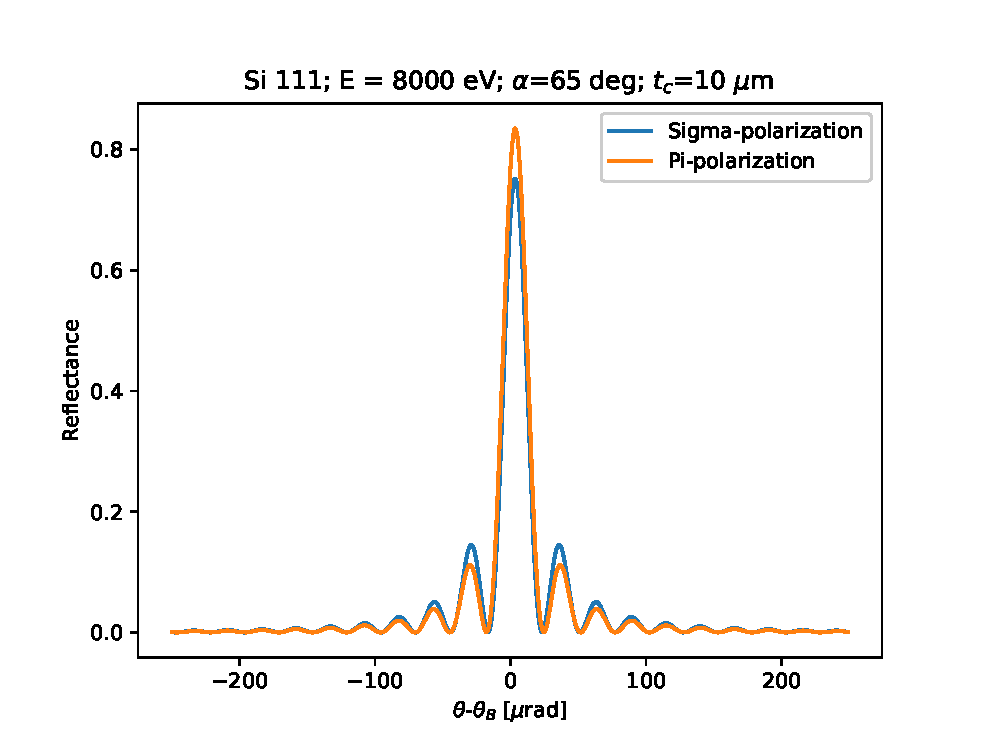
\includegraphics[width=0.49\textwidth]{figures/Laue_1.eps}
    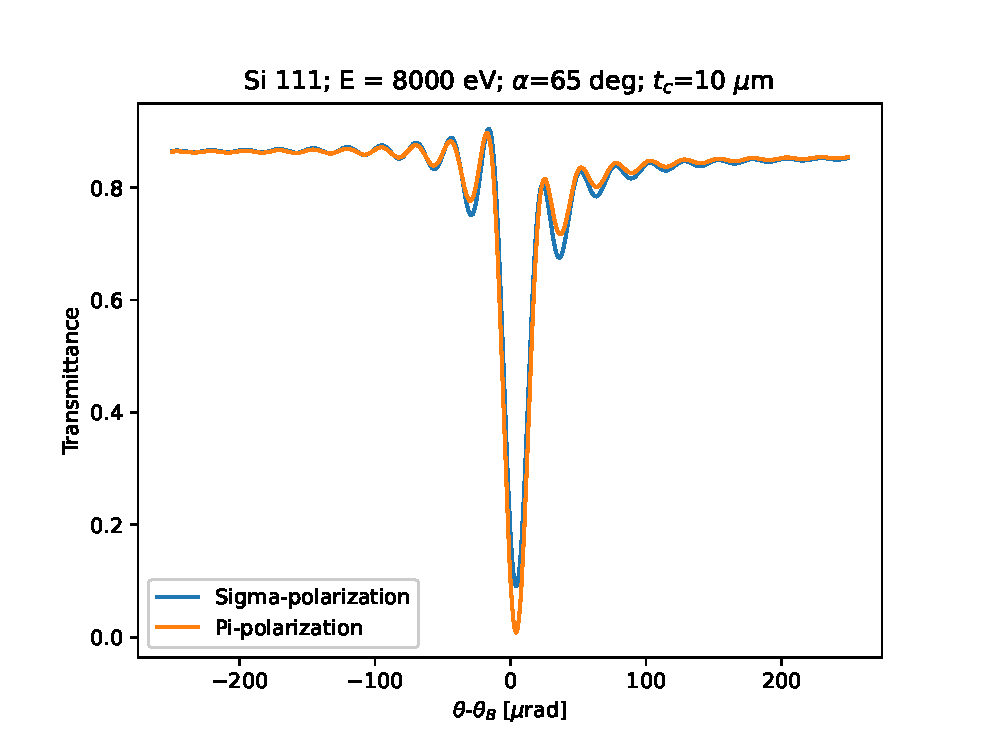
\includegraphics[width=0.49\textwidth]{figures/Laue_2.eps}
    \caption{Example of reflectance and transmittance for a Laue Si 111 crystal.}
\end{figure}

\inblue{
\todo{add intro? verify? clarify?} Note that $a, u_0, \omega$ in equations~(\ref{eq:lauerandt}) are complex. The careful look at the real and imaginary parts conducts to common expressions for absorption and Pendell\"osung. The real part of the exponential argument gives a pure absorption term:  
$\exp(\operatorname{Re} i s (u_0+\omega))$. Using $u_0 + \omega = (1/2)[b(u_0+\alpha')+u_0]$, we find
\begin{subequations}
\begin{align}
    \exp(\operatorname{Re} i s (u_0+\omega)) = \nonumber \\
    \exp[\operatorname{Im} s (u_0+\omega)] = \inred{??} \nonumber\\
    \exp[T \gamma_0 \large( \frac{1}{\gamma_0} + \frac{1}{\gamma_h} \large) \operatorname{Im} u_0] = \nonumber \\
    \exp[-\frac{\lambda}{\pi} \frac{t_c}{2} \large( \frac{1}{\gamma_0} + \frac{1}{\gamma_h} \large) \operatorname{Im} \chi_0].
\end{align}
\end{subequations}
The Pendell\"osung comes from the pure oscillation of $|\sin(as)|^2$ \inred{in in equations~(\ref{eq:lauerandt}a and b??)}. Knowing the identity $|\sin(x+iy)|^2=\sin^2x + \sinh^2 y$, we get the Pendell\"osung distance along $s_0$ as 
\begin{equation}
    \Lambda = \frac{\pi}{\operatorname{Re} a}=\frac{\lambda}{\operatorname{Re}\sqrt{b\chi_h\chi_{-h} + w^2}},
\end{equation}
which depends on $\theta$. At $\theta=\theta_c$ we find the usual value $\Lambda=\lambda/(\operatorname{Re}\sqrt{b \chi_h \chi_{-h}})$ 
}


%%%%%%%%%%%%%%%%%%%%%%%%%%%%%%%%%%%%%%%%%%%%%%%%%%%%
%
%%%%%%%%%%%%%%%%%%%%%%%%%%%%%%%%%%%%%%%%%%%%%%%%%%%%
\subsection{Bragg case}
\label{sec:TTsolutionsBragg}

For the Bragg case $b<0$. Considering $T$ the path length of the incident beam in the crystal, and a ``normalized" incident beam $D_0(0)=1$. The other boundary condition is found at the bottom surface, where there is no diffracted field in the ascendant direction $D_h(T)=0$. Knowing $(D_0(0),D_h(T)) = (1,0)$, we have the unknows $(D_0(T),D_h(0))$ and we have to modify  the transfer equation~(\ref{eq:Mtransfer}) to get the ``Bragg case scattering matrix" $S$

\begin{equation}\label{eq:scatteringMatrix}
    \begin{pmatrix}
    D_0(T)\\
    D_h(0)
    \end{pmatrix}
    =
    S
        \begin{pmatrix}
    D_0(0) \\
    D_h(T)
    \end{pmatrix}
    =
    \begin{pmatrix}
    s_{11} & s_{12}\\
    s_{21} & s_{22}
    \end{pmatrix}
    \begin{pmatrix}
    D_0(0) \\
    D_h(T)
    \end{pmatrix}
        =
    \begin{pmatrix}
    m_{11}-\frac{m_{12} m_{21}}{m_{22}} & \frac{m_{12}}{m_{22}}\\
    -\frac{m_{21}}{m_{22}} & \frac{1}{m_{22}}
    \end{pmatrix}
    \begin{pmatrix}
    D_0(T) \\
    D_h(0)
    \end{pmatrix}.
\end{equation}


The amplitudes are, after a simple algebraic calculations,  using $D_0(0)=1$ and $D_h(T)=0$, are
\begin{subequations}
\label{eq:braggrandt}
\begin{empheq}[box=\fbox]{align}
r = D_h(0)=s_{21}=
\frac{-i b u_h \sin(a T)}{a \cos(a T) + i \omega \sin(a T)}\\
t = D_0(T)=s_{11}=
\frac{a~\exp(i T(u_0+ \omega))}{a \cos(a T) + i \omega \sin(a T)} ,
\end{empheq}
\end{subequations}

The diffraction profiles are $\mathcal{R}=|r|^2 P$ (diffracted intensity or reflectance) and $\mathcal{T}=|t|^2$ (forward diffracted intensity or transmittance).
An example is in Fig.~\ref{fig:braggProfiles}. 

\begin{figure}\label{fig:braggProfiles}
    \centering
    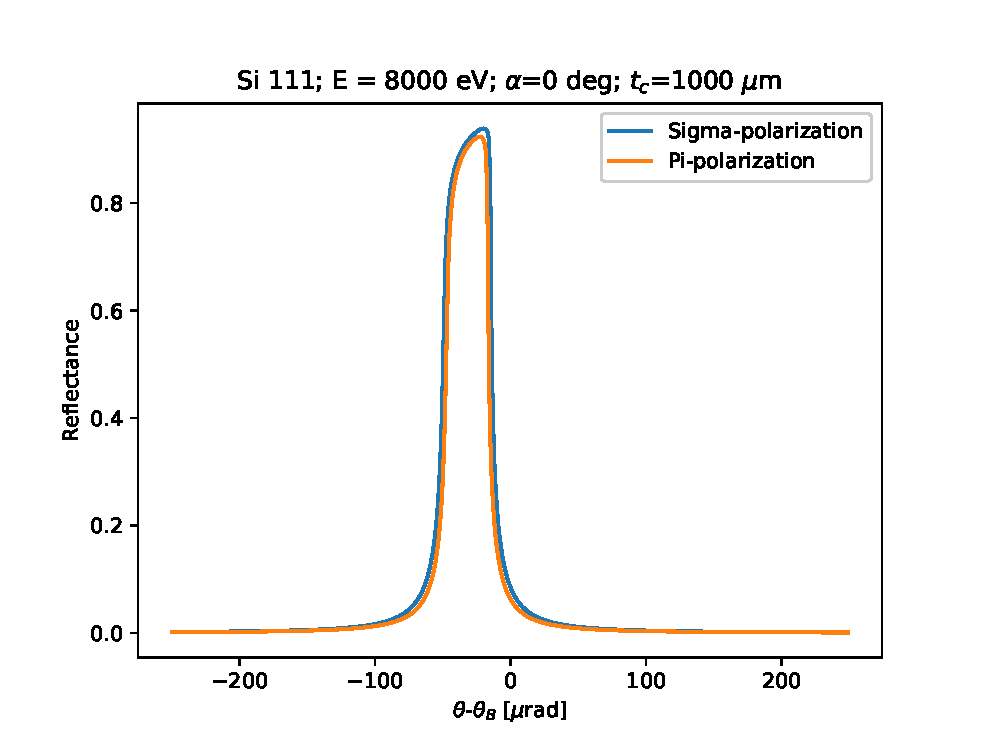
\includegraphics[width=0.49\textwidth]{figures/Bragg_1.eps}
    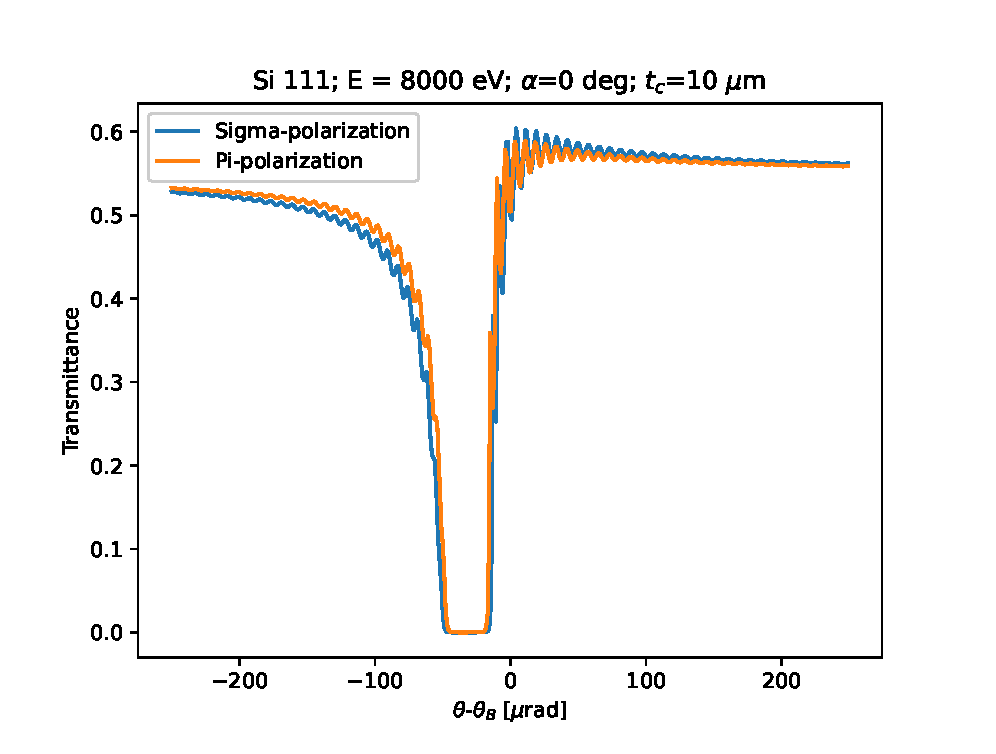
\includegraphics[width=0.49\textwidth]{figures/Bragg_2.eps}
    \caption{Example of reflectance and transmittance for a Bragg Si 111 crystal of $t=$\SI{10}{\micro\meter} at 8 keV. }
\end{figure}

\inred{
It may be interesting to calculate the field inside the crystal, i.e. $D_0(s)$ and $D_h(s)$. Introducing the coefficients in (\ref{eq:TTbraggCoefficients}) into equations (\ref{eq:BSolutions}) we obtain, after some algebraic manipulation
\begin{subequations}\label{eq:bragginside}
\begin{align}
D_h(s)&=\frac{i b u_h \sin(as - aT)}{a \cos(aT) + i \omega \sin(aT)} e^{is(u_0+\omega)}\\
D_0(s)&= \frac{a \cos(as-aT) - i \omega \sin(as-aT)}{a \cos(aT) + i \omega \sin(aT)} e^{is(u_0+\omega)}.
\end{align}
\end{subequations}
}
\inblue{
An example of simulation of the field inside the crystal using equations~(\ref{eq:bragginside}) is in Fig.~\ref{fig:braggMap}. For the Laue case, also shown in this figure, we observe that the field at coordinate $s$ is simply calculated by the equations~(\ref{eq:lauerandt}) replacing $T$ by $s$. 
}

\begin{figure}\label{fig:braggMap}
    \centering
    \includegraphics[width=0.49\textwidth]{figures/Bragg_DH.png}
    \includegraphics[width=0.49\textwidth]{figures/Bragg_D0.png}
    \includegraphics[width=0.49\textwidth]{figures/Laue_DH.png}
    \includegraphics[width=0.49\textwidth]{figures/Laue_D0.png}
    \caption{Examples of electric field intensity inside the crystal as a function of the 
    deviation angle $\theta-\theta_B$ and thickness ratio $-s/T$ for a symmetric Si 111 at 8 keV with thickness $t=$\SI{50}{\micro\meter} in Bragg or Laue geometry. 
    a) Bragg $|D_h|^2$, b) Bragg $|D_0|^2$,
    c) Laue $|D_h|^2$, d) Laue $|D_0|^2$.
    \todo{Change the titles for consistency}
    }
\end{figure}



\todo{REMOVE THIS? OR COMPLETE THE CASE OF ZERO ABSORPTION? A particular case is to consider zero absorption. 
$a^2$ is real negative \todo{Why?} if $|\theta-\theta_c|<|\chi_h|/(|b|^2 \sin(2 \theta_B))$, then $aT=i |a| T$, $\cos(a T)=\cosh(|a|T)$, $\sin(a T)=i \sinh(|a|T)$, 
\begin{equation}
    r = \frac{b u_h \sinh(|a|T)}{i |a|T \cosh(|a|T)- \omega
    \sinh(|a|T)}=
\frac{i |b| u_h \tanh(|a|T)}{|a|+ i \omega \tanh(|a|T)}.
\end{equation}
For $t \rightarrow \infty$, 
\begin{equation}
    r \rightarrow - \frac{i \inred{|b|} u_h}{|a|+ i \omega} .
\end{equation}
}

\inblue{
The matrix method permits to obtain the complex reflection and transmission amplitudes of a crystal made by layers of different crystals (or the same crystal with different orientations). For that,
i) construct the transfer matrix of the total crystal by multiplication of the transfer matrices of the different layers (each one calculated using equations~[\ref{eq:scatteringMatrix })];
ii) if geometry is Laue, obtain reflectance and transmittance using the coefficients $m_{21}$ and $m_{11}$ of this matrix [equation~(\ref{eq:lauerandt})], respectively; otherwise (Bragg geometry), compute the scattering matrix using equation~(\ref{eq:scatteringMatrix}) and reflectance and transmittance are given in the coefficients $s_{21}$ and $s_{11}$ [equation~(\ref{eq:braggrandt})], respectively.  This method can be used for analyzing distorted and bent crystals.
}\todo{example? Or better leave this for a future work...}

\inblue{In the case where the incident beam enters the crystal by the bottom surface, we set $(D_0(0),D_h(T))=(0,1)$ in equation~(\ref{eq:scatteringMatrix }) and  we obtain the amplitudes $\bar{r}=D_0(T)=s_{12}; \bar{t}=D_h(0)=s_{22}$, where the bar indicates ``from bottom to top". This allows, for example, to calculate the reflectivity $r_{2}$ of a crystal of double thickness $2 T$ using the scattering matrix of the crystal of thickness $T$
by using the infinite sum $r_2=r(1 + (t \bar{t} / (1-r \bar{r})))=s_{21}(1 + (s_{11} s_{22} / (1-s_{21} s_{12})))$. This can be checked both analytically and numerically\footnote{See, for example, the example {\tt Si111\_layered.py} in {\tt crystalpy}.} (see Fig.~\ref{fig:doublelayer}).
}

\begin{figure}\label{fig:doublelayer}
    \centering
    \includegraphics[width=0.49\textwidth]{figures/figlayered2.pdf}
    \includegraphics[width=0.49\textwidth]{figures/doublelayer2.png}
    \caption{Example of calculation of the reflection amplitude $r_2$ of a Si 111 crystal of \SI{2}{\micro\meter} thickness $2T$ from the amplitudes of the half-layer (\SI{1}{\micro\meter}) of thickness $T$. $r_2$ can be obtained as an infinite sum $r_2 = r + r t \bar{t} + r t \bar{t} (r \bar{r}) + r t \bar{t} (r \bar{r})^2 + ...= r[1 + t \bar{t}\sum_{n=0}^{\infty}(r\bar{r})^n]=r(1 + (t \bar{t} / (1-r \bar{r})))$. Photon energy is 8 keV.
    }
\end{figure}

% \section{Scattering and transfer matrices}
% \label{sec:matrices}

% Equations (\ref{eq:BSolutions}) represent a system of two equations containing two coefficients $c_1$ and $c_2$ and two fields ($B_0$ and $B_h$) that are latter expressed at the top ($s=0$) and bottom ($s=T$) surfaces. From these four fields, we can calculate two as a function of the other two. In the usual case, we calculate the diffracted and transmitted fields at the corresponding exit surface (which depends on the geometry, Bragg or Laue) given the other two that are set as boundary conditions. This gives the ``scattering matrix". In other cases, when one considers a complex crystal made by several piled individual crystal layer, we would be interested in calculating the diffracted and transmitted beam at the bottom as a function of the beams from the top.   

% \subsection{Scattering matrix in Bragg case}
% For the Bragg case, we calculate $D_0(T)$ (transmitted) and $D_h(0)$ (diffracted) as a function of generic $D_0(0)$ and $D_h(T)$, so we can write in matrix form
% \begin{equation}
%     \begin{pmatrix}
%     D_h(0)\\
%     D_0(T)
%     \end{pmatrix}
%     =
%     S
%         \begin{pmatrix}
%     D_0(0) \\
%     D_h(T)
%     \end{pmatrix}
%     =
%     \begin{pmatrix}
%     s_{11} & s_{12}\\
%     s_{21} & s_{22}
%     \end{pmatrix}
%     \begin{pmatrix}
%     D_0(0) \\
%     D_h(T)
%     \end{pmatrix},
% \end{equation}
% where the terms of the scattering matrix $S$ are 
% \begin{subequations}\label{eq:scatteringMatrix }
% \begin{align}
% s_{11} &= \frac{-i b u_h \sin(a T)}{a \cos(a T) + i \omega \sin(a T)};\\
% s_{12} &= \frac{a~\exp(-i T (u_0+ \omega))}{a \cos(a T) + i \omega \sin(a T)};\\
% s_{21} &= \frac{a~\exp(i T (u_0+ \omega))}{a \cos(a T) + i \omega \sin(a T)};\\
% s_{22} &= \frac{-i u_{-h} \sin(a T)}{a \cos(a T) + i \omega \sin(a T)}.
% \end{align}
% \end{subequations}


% For the case studied in section~\ref{sec:TTsolutionsBragg} we set $(D_0(0),D_h(T))=(1,0)$ from there we get $s_{11}=r; s_{21}=t$, with $r$ and $t$ from equations (\ref{eq:braggrandt}). 

% % Similarly, when the incident beam enters the crystal by the bottom surface, as studied in appendix~\ref{sec:braggfromtheback}, we set $(D_0(0),D_h(T))=(0,1)$ and  we get $s_{12}=\bar{r}; s_{22}=\bar{t}$, with $r$ and $t$ from equations (\ref{eq:braggrbarandtbar}) \todo{suppress the appendix?}.

\inblue{
\subsection{Thick crystal approximation}\label{sec:thick}
}

\inblue{
Equations~(\ref{eq:lauerandt}) and (\ref{eq:braggrandt}) are expressed in terms of $a$, but it is clearly seen that they depend only on $a^2=bu_h u_{-h}+\omega^2$ which is a complex number. Let us choose $a$ such that $\operatorname{Im}(a)>0$. Then  
$\exp(iaT)=\exp[iT\operatorname{Re}(a)-T\operatorname{Im}(a)]\rightarrow 0$, as $T\rightarrow \infty$; consequently $\sin(aT)\approx \inred{-}(i/2) \exp(-i a T)$, $\cos(aT)\approx (1/2) \exp(-i a T)$. The reflectivity of the Bragg case [equation~(\ref{eq:braggrandt}a)] take a simplified form
\begin{equation}\label{eq:thickbraggr}
    r = \frac{b u_h}{a-\omega} = \frac{a+\omega}{u_{-h}},
\end{equation}
where $a$ can be obtained from $a^2$ as: 
\begin{equation}
a = \frac{1}{\sqrt{2}} \left[ \frac{\operatorname{Im}(a^2)}{\sqrt{|a^2|-\operatorname{Re}(a^2)}} + i \sqrt{|a^2|-\operatorname{Re}(a^2)} \right].
\end{equation}

Equation~(\ref{eq:thickbraggr}) is a useful result, as most crystal monochromators used in synchrotron radiation are thick crystals in Bragg (reflection) mode. For all other geometries (Bragg transmission, and both Laue cases) the approximation $T\rightarrow \infty$ makes the exponential term tends to zero, therefore there is no intensity at the back crystal surface. If we apply the approximations mentioned, but leave the exponential term (with a reasonable small $T$, thus small absorption), we obtain diffraction intensity distributions that do not present Pendell\"osung. The simplified form of equation~ (\ref{eq:braggrandt}b) is   
\begin{equation}\label{eq:thickbraggt}
    t = \frac{2a}{a-\omega} e^{i T (u_0+\omega+a)},
\end{equation}
and for the Laue case [equations (\ref{eq:lauerandt}b)] we get
\begin{subequations}
\label{eq:thicklaue}
\begin{align}
r = & - \frac{b u_h}{2 a} e^{iT (u_0+\omega-a)}  \\
t = & \frac{1}{2} (1 + \frac{\omega}{a})e^{i T (u_0+\omega-a)}.
\end{align}
\end{subequations}
}

\todo{
\begin{itemize}
    \item a high numerical precision is required for calculating $\sin(aT)$, $\cos(aT)$ and $\exp(iT(u_0+\omega))$ for large values of T. This is  a typical problem when calculating Bragg reflection case using a large $t_c$. Can we make a recipe to switch to the "thick" crystal model for $t_c>t_{\text{eff}}$. How to calculate $t_{\text{eff}}$? 
\end{itemize}
}
\inblue{
\subsection{The direction of the incident and diffracted waves}\label{sec:directions}
}
\inblue{
As mentioned before, the selection of the directions used to solve the TT equations contains some dose of arbitrarily. In our choice, $\textbf{k}_0$ vector corresponds exactly with the direction and wavelength of the incident ray or wave, which is not necessarily verifying the Bragg law.
The vector $\textbf{k}_h$ (see section~\ref{sec:TT}) is defined as as $\textbf k_h=\textbf k_0 + \textbf h$. Therefore, it is not necessarily matching the wavevector of the outgoing ray or wave outside the crystal.
In many applications, like in ray tracing, it is essential to know the output wavevector $\textbf{k}_{\text{out}}$ that exits from the crystal. The length of $\textbf{k}_h$ is [equation~(\ref{eq:alpha})] $|\textbf{k}_h|=k\sqrt{1-\alpha}$.
To get $\textbf{k}_{\text{out}}$ we must get into account i) its length is the same as $\textbf{k}_0$, and ii) its value parallel to the crystal surface $\textbf{k}_{\text{out}, ||}$ must be equal to $\textbf{k}_{h,||}$ (continuity of the tangential component of the electric field at the crystal-vacuum interface).
These conditions permit to determine how the perpendicular component of $\textbf{k}_{\text{out}}$ differs from $\textbf{k}_h$
\begin{equation}
    \textbf{k}_{\text{out}, \bot} = \kappa \textbf{k}_{h,\bot},
\end{equation}
with 
\begin{equation}
    \kappa^2 = \frac{|\textbf{k}_0|^2-|\textbf{k}_{h,||}|^2}
    {|\textbf{k}_{h,\bot}|^2}
\end{equation}
}

\todo{simplify the discussion? Write $\textbf{k}_{\text{out}, \bot} = \text{something} \times \textbf{n}$? }

\todo{ something still not clear:

The formulation done is ``inside the crystal". Therefore $D_{0,h}(0)$ corresponds to the field ``inside" the crystal. So, $D_0(0)=1$ is the amplitude of the incident plane wave inside the crystal. 
And $\Psi_0(0)=D_0(0) e^{i \textbf{k}_0. \textbf{r}}$ with $\textbf{k}_0$ outside the crystal. This may be confusing but it is just definitions.  
Right? 

Having $\Psi(\textbf r) = D_0(\textbf r) e^{i \textbf k_0 . \textbf r} + D_h(\textbf r) e^{i \textbf k_h . \textbf r}$ this implies $\Psi(s) = D_0(s) e^{i \textbf k_0 . \textbf{s}} + D_h(s) e^{i \textbf k_h . \textbf s}$ with $\textbf{s}=(s_0,s_h)$. Can we write $\Psi(s)=\Psi_0(s)+\Psi_h(s)$?


For the output beam (in Bragg), we calculate $D_h(0)$ inside the crystal. The direction of the scattered wave is $\textbf{k}_{\textbf{out}}$ as defined before. 
Is it really necessary to use the conservation of the parallel component of the diffraction $\textbf{h}_{\textbf{out},||}= \textbf{k}_{0,||} + \textbf{h}_{||}$? Or, can it be deduced in another way, like using  $\nabla  \arg(\Psi_h(0))$? 

Other things: 
\begin{itemize}
    \item discuss the fact that $b$ is not constant.
    \item may be: make a comment for the grazing incidence case (\cite{Yashiro2001, Stepanov1998})
\end{itemize}
}

\inred{
\subsection{Application to multilayers}
}\label{sec:multilayers}


\todo{REMOVE THIS SECTION. LEFT FOR THE FUTURE?

Can we directly apply the amplitudes in (\ref{eq:braggrandt}) to a multilayer? It is enough to replace $\chi_0$ by the averaged $\bar{\chi}=n^2-1$ and $\chi_h$ by $\chi_1$ and $\chi_{-h}$ by $\chi_{-1}$? Is this a bilayer? Shall we then use the scattering matrix? 
Can we use $\alpha=2(\theta-\theta_B)\sin(2\theta_B)$ ?
See also \cite{Osterhoff2012,Osterhoff2013}.

Some possible ideas for the matrix methods
\begin{itemize}
    \item the multilayer case:
    \begin{itemize}
        \item relation between scattering and transfer matrices for multilayers. We can build a multilayered $M=\Pi M_i$ and then calculate its corresponding scattering matrix?
        \item Connection with the Parratt recursion formula
        \item transition layer (non-abrupt change, see \cite{Lobach})
        \item Roughness layer
    \end{itemize}and 
    \item may be: discuss the roughness layer

\end{itemize}
}

\inred{
\subsection{OTHER SECTIONS?}
}

\todo{
\begin{itemize}
    \item Discuss the differences of the presented theory with Darwin (see \cite{Yashiro2000, Yashiro2001}), Ewald (??), Zachariasen (none, as seen in Appendix~\ref{appendix:zachariasen}), etc. 
\end{itemize}
}
% \begin{figure}\label{fig:2T}
%     \centering
%     \includegraphics[width=0.49\textwidth]{figures/fig2T.png}
%     \caption{A $2T$ crystal made with two $1T$ crystals. \todo{replace $r'$ by $\bar r$ and $t'$ by $\bar t$}}
% \end{figure}

% As a consistency test, we consider a single Bragg crystal of $s=2T$ made by two piled crystals of $T$. The reflectance $r_{2T}$ of the 2$T$ crystal is (see Fig.~\ref{fig:2T})
% \begin{equation}
%     r_{2T} = r+t r \bar t  \sum_{n=0}^\infty (r \bar r)^n =r + \frac{t r \bar t}{1-r \bar r} = r \frac{1-r \bar r + t \bar t}{1-r \bar r}
% \end{equation}


% We define $b=\sin\theta_0/\sin\theta_h$ ($\theta_{0,h}$ the grancing angles of the incident and reflected directions with respect to the crystal surface, and $s=s_0+s_h/b$. Unlike the usual convention, we have $b>0$. The crystal surface has equation $s=0$. 

% The refractive wave is such that $D_0^{\text{ref}}=\exp(u_0 s_0) f(s_h)$, with $D_0^{\text{ref}}(s_h/b,s_h)=1$; therefore $\exp(i u_0 s_h/b)=1$ and $D_0^{\text{ref}}=\exp(i u_0 (s_0 - s_h/b) )=\exp(i u_o s)$; this implies $Im(u_0)>0$.


% The TT equations are then
% \begin{subequations}
% \label{eq:TTlaue}
% \begin{align}
% D'_0(s) =& i u_0 D_0(s) + i u_{-h} D_h(s); \\
% D'_h(s) =& -i b (u_0 + \alpha') D_h(s) - i b u_{h} D_0(s).
% \end{align}
% \end{subequations}

% We introduce the functions $B_{0,h}(s)$ by setting
% \begin{equation}
% \label{eq:TTbraggB}
% D_{0,h} = \exp \left( i s \frac{u_0 - b (u_0+\alpha')}{2} \right) B_{0,h} = \exp(i s (u_0-\omega)) B_{0,h},  
% \end{equation}
% with $\omega=(b(u_0+\alpha')+u_0))/2$. 

% \inblue{Note that $\exp(i s (u_0 - \omega))=\exp(-s(1+b)/2+ b \alpha/2))=\exp(-s(1+b)/2+ b \sin(2 \theta_B) (\theta - \theta_c)))$, with the corrected value of the Bragg angle $\theta_c=\theta_s - \frac{(1+b) Re(\chi_0)}{2 b \sin(2 \theta_B)}$
% }



% They are solutions of 
% \begin{subequations}
% \begin{align}
% B'_0(s) =& -i \omega B_0(s) + i u_{-h} B_h(s); \\
% B'_h(s) =& i \omega B_h(s) + i b u_{h} B_0(s).
% \end{align}
% \end{subequations}


%%%%%%%%%%%%%%%%%%%%%%%%%%%%%%%%%%%%%%%%%%%%%%%%%%%%
%
%%%%%%%%%%%%%%%%%%%%%%%%%%%%%%%%%%%%%%%%%%%%%%%%%%%%
\section{The {\tt crystalpy} library}
\label{sec:crystalpy}

{\tt Crystalpy} is a Python library which performs calculations on diffraction
from perfect crystals using the formalism introduced in the previous chapters. It also simulates the changes in the polarization state of the x-ray beam brought
about by the diffraction using Müller-Stokes formalism. The first version of this library was developed by Edoardo Cappelli, Mark Glass and Manuel Sanchez del Rio. 
As mentioned in section~\ref{sec:Intro}, many software tools are available for crystal calculations based on the dynamical diffraction theory. However, these are usually complex ancient code, which makes complicate the use, integration and maintenance in new applications. For this reason, we wanted to create a modern, extensible, well-documented, and friendly library. It will help in the future as support for new versions of the codes delivered in platforms like OASYS \cite{codeOASYS}. 

The {\tt crystalpy} library is written in the python language and uses standard libraries (numpy and scipy).
It basically contains three
packages: {\tt util}, {\tt diffraction} and {\tt polarization}.
The {\tt util} toolbox contains auxiliary classes which take part in the diffraction
process but have their own significance independently of it.
 The {\tt Vector} class includes definition and operations (addition, scalar product, cross product, normalization, rotation around
an axis etc) of a 3D vector. 
% This object is fundamental as the whole library was written with the idea of making everything work with vectorial quantities instead of using angles. 
% To clarify the advantages of this approach, let us imagine we have an x-ray beam impinging on the surface of a crystal at an angle $\theta$ with respect to the normal: how do we describe this in the code? The simplest way would be to identify its direction by assigning $\theta$ to a variable, e.g. {\tt angle\_with\_normal}, while a more complicated way would be to use an object-oriented approach and write:
% \texttt{normal = Vector(0, 0, 1) \# z axis}
% \texttt{beam\_direction = normal.rotateAroundAxis(Vector(1, 0, 0), theta) }
% This is more cumbersome, both at design and run time, but it allows for a very straightforward manipulation of the vectors: if, for example, we wanted to know the angle between the beam direction and the reciprocal vector \textbf{H}, we would also have to keep track of the angle between \textbf{H} and the normal and pay attention to the sign of the angles in order to avoid mistakes. The object-oriented approach becomes even more advantageous in a three-dimensional system, where storing one angle is not enough and finding the angle between vectors that do not share the same plane with the normal can be quite a head-scratcher\footnote{The {\tt rotateAroundAxis} function is implemented using Rodrigues formula (see Wikipedia)}.
The {\tt Photon} class is a minimum class for a photon, containing the energy (in eV) and a unit direction vector. Superclasses of Photon are {\tt ComplexAmplitudePhoton} (that contains the complex amplitude for $\sigma$ and $\pi$ polarizations), and {\tt PolarizedPhoton} with the four Stokes parameters.

% as class attributes and contains a method for calculating the degree of circular
% polarization, defined as $P_c = S_3 /S_0$.} attribute. 
% It is an abstraction of a monochromatic plane wave rather than of a physical photon.
% Both {\tt Photon} and {\tt PolarizedPhoton} 
The photon classes 
have corresponding {\tt PhotonBunch} objects, which group a collection of photons. The interest of using these classes is for vectorizing operations and reducing computational time. For the calculations, vectors are always preferred to angles. Typical angle or photon scans as shown in Fig.~\ref{fig:braggProfiles} are calculating defining a $\tt Photon$ entity for each point, group then in a {\tt PhotonBunch} for being send to the crystal. 
% \footnote{the term photon will be used here to refer to a Photon object even if it does not correspond to a physical photon}, this means it can be indexed and called iteratively by using the in keyword:
% {\tt
% for photon in PhotonBunch:
%     do\_something()
% }
% These classes are used as ``beam" or ``signal" between different widgets
% when integrating the library into OASYS.


The {\tt DiffractionSetup} toolbox is twofold: i) as a container of physical parameters of the crystal and the definition of the crystal setup, and ii) supply methods to calculate important physical quantities needed in the calculation, in particular the structure factors. The {\tt DiffractionSetup} class handles the information about the crystal setup and collects all the parameters needed to fully define the physical system we are modelling:
{\tt geometry\_type} (among {\tt BraggDiffraction, BraggTransmission, LaueDiffraction} and {\tt LaueTransmission}),
{\tt crystal\_name} (a string, e.g. Si, Ge),
{\tt thickness} (crystal thickness in SI units [m]),
{\tt miller\_h(,k,l)} (the Miller indices),
and {\tt asymmetry\_angle} (angle in degrees between the crystal surface and the planes $hkl$ as defined in \cite{codeCRYSTAL}, shown in figure~\ref{fig:edo_sketch}).
% Let us explore this toolbox and see how the computation is handled.


% \begin{enumerate}
 
% \begin{itemize}

%     \item {\tt geometry\_type} clarifies which is the diffraction geometry among {\tt BraggDiffraction, BraggTransmission, LaueDiffraction} and {\tt LaueTransmission}.
%     \item {\tt crystal\_name} is a string (e.g. Si, Ge . . . ) specifying which crystal is being used for the diffraction.
%     \item {\tt thickness} of the crystal in centimetres; we are considering parallel plane plates, so this parameter is always well defined.
%     \item {\tt miller\_h(,k,l)} are the Miller indices identifying the family of lattice planes which satisfy the Laue condition. Remember that in the two-wave approximation only one family of planes takes part in the diffraction process, so three indices are enough to fix the \textbf{H} vector once the crystal structure is known.
%     \item {\tt asymmetry\_angle} is shown graphically in figure~\ref{fig:edo_sketch} and is the angle between the crystal surface and the planes $hkl$ as defined in XX. It depends on how the crystal has been cut.
% \end{itemize}


\begin{figure}
    \centering
    \includegraphics[width=0.8\textwidth]{figures/edo_sketch.png}
    \caption{Schematic drawings of Bragg (left) and Laue (right) diffraction setups: \textbf{H} is the reciprocal vector associated with the $hkl$ family of lattice planes, also called the Bragg normal, $\theta_B$ is the Bragg angle and $\alpha_X$ is the asymmetry angle as defined in \cite{codeCRYSTAL}.
    \todo{change vector format (from arrows to bold)} }
    \label{fig:edo_sketch}
\end{figure}

The {\tt DiffractionSetup} class has methods to access the basic information of the crystal (defined as a string, e.g. ``Si") such as {\tt angleBragg}, {\tt dSpacing}, and {\tt unitCellVolume}, and very important, to compute the structure factors: {\tt F0}, {\tt FH}, {\tt FH\_bar}. These parameters can be obtained from several libraries external to {\tt crystalpy}. We implemented two options: i) {\tt DiffractionSetupXraylib} using the {\tt xraylib} library \cite{xraylib}, and ii) {\tt DiffractionSetupDabax} that uses the DABAX library \cite{dabax}. This modular structure permits disconnecting the calculation part from the access to optical and physical constants. Indeed, the implemented structure permits us to easily implement other sources of these data. As an example, we could also use pure text files thus not needing to import the {\tt xraylib} or {\tt dabax} packages. We implemented this for the crystal material files of the SHADOW~\cite{codeSHADOW} code.

% It takes advantage of the functions implemented in the xraylib library XXX to provide methods able to yield important parameters such as the Bragg angle at a certain energy: angleBragg(energy), the structure factor Fourier components \textbf{F\_0} , \textbf{F\_H} and \textbf{F\_$\bar{H}$}: \textbf{F0(energy)}, \textbf{FH(energy)},
% \textbf{FH\_bar(energy)}, the unit cell volume: \texttt{unitCellVolume()}, the lattice
% spacing for the $hkl$ family of planes: \texttt{dSpacing()} and the reciprocal
% vector \textbf{H}: \texttt{normalBragg()}. 

% If one just wants to plot the reflectivities/trasmittivities as functions of angular deviation or energy (like in figures \ref{fig:braggProfiles}, \ref{fig:laueProfiles}) the {\tt DiffractionSetupSweeps} class can be used to build a {\tt PhotonBunch} containing all the photons for whom the calculations are going to be carried out. 
% It needs to know how many photons to create and in which angular and/or energy range, so it takes as attributes {\tt energy\_min}, {\tt energy\_max}, {\tt energy\_points} for the energy and {\tt angle\_deviation\_min}, {\tt angle\_deviation\_max} and {\tt angle\_deviation\_points} for the angular deviations from the (0, 1, 0) direction.

% \item The {\tt Diffraction} class manages the computations without actually doing anything at initialization. It behaves as an administrator, directing the inputs to where they are needed and collecting the results in an orderly fashion to create the output. 
% % The advantage of this solution is that, in order to compute the results from the main, an Orange widget or a user script, one only needs to do this:

% \begin{verbatim}

% diffraction = Diffraction()
% outgoing_photon_bunch = diffraction.calculateDiffractedPhotonBunch(diffraction_setup,
% incoming_photon_bunch)

% \end{verbatim}
% The {\tt calculateDiffractedPhotonBunch} method iterates over all the
% photons in the incoming bunch and for each one calls the {\tt calculate-DiffractedPhoton} function. This in turn creates an instance of the {\tt PerfectCrystalDiffraction} class. This class contains methods to perform the actual calculations. This matryoshka-like structure is illustrated in figure~\ref{fig:edo_matryshka}. Diffraction is designed to propose different methods of calculation, or different algorithms. At present, only Guigay (this formalism) and Zachariasen theories for perfect crystals are available.

The {\tt Diffraction} class contain methods to drive the simulations, thus using both {\tt DiffractionSetup} and {\tt PhotonBunch} and calculates the reflectivities and output photons. It is merely an interface to call the different classes that calculates the different kind of crystal models. For the moment, only flat perfect crystals are implemented in the {\tt PerfectCrystalDiffraction} class implementing the formulation and theory presented in section~\ref{sec:TTsolutions}. The {\tt PerfectCrystalDiffraction} class handles the actual computations. It calculates the diffraction parameters by means of
several methods and then plugs them into the equations XXX according to the specified experimental geometry: for each
one setup the results are two amplitude ratios for the two polarization
states {\tt S} (i.e. $\sigma)$) and {\tt P} (i.e $\pi$) \todo{better define. Indeed, this is the complex amplitude with the square root of the power factor $\sqrt{P}$}. A graphical representation of the steps
of the calculation is shown in figure \ref{fig:edo_matryoshka}.



% \begin{figure}
%     \centering
%     \includegraphics[width=0.7\textwidth]{figures/edo_structure.png}
%     \caption{Structure and data flow of the Diffraction class. The {\tt \_checkSetup} method checks whether the parameters from {\tt DiffrationSetup} are not contradictory, e.g. it verifies that, if the declared geometry type is Bragg, the asymmetry angle be smaller than the Bragg angle (why it must be so becomes clear by inspecting figure \ref{fig:edo_sketch}); if this is not true, then the angles are not compatible with the expected geometry and an exception must be raised. We will see when dealing with the polarization toolbox that the amplitudes are used to generate a ``polarized photon" as output. The $\Psi$ parameters are computed via equation XXX}
%     \label{fig:edo_structure}
% \end{figure}




\begin{figure}
    \centering
    \includegraphics[width=0.4\textwidth]{figures/edo_matryoshka.png}
    \caption{A board-game-style representation of the calculation process in {\tt crystalpy}. The letters stand for the parameters computed using the equations we have derived in section \ref{sec:TTsolutions}. Each one of the concentric circles is one ``layer" of computation, i.e. the innermost parameters are computed starting from the parameters surrounding them on the outside. 
    For example, to obtain $z$ using equation XXX we need $b$, $\Psi_0$  and $\alpha$, which are adjacent to $z$ and located further out; to compute $x_{1,2}$ via XXX we need $z$, $q$, $\Psi$, \textbf{H} and $P$, and so on. \todo{adapt to our notation. Define code color relative to the class.}}
    \label{fig:edo_matryoshka}
\end{figure}


% \subsection{The {\tt polarization} toolbox}

% This toolbox is made up of classes needed to allow {\tt Diffraction} to perform
% polarization calculations through class methods such as {\tt calculateDiffracted-PolarizedPhotonBunch} and {\tt calculateDiffractedPolarizedPhoton}, which follow the same process described in figure~\ref{fig:edo_structure} but have {\tt PolarizedPhoton}
% objects as inputs and outputs. These functions compute {\tt photon\_out} and
% amplitudes through the dedicated {\tt PerfectCrystalDiffraction} methods and then use the field amplitudes to build the Müller matrix for a crystal
% phase plate. The matrix is then applied to the Stokes vector attribute of
% the incoming {\tt PolarizedPhoton} object to get the outgoing polarized photon.
% The single Stokes parameters can then be extracted and plotted as a function of angular deviation from the Bragg angle to analyse the birefringence
% of the crystal phase plates.

% To do this the toolbox contains:
% \begin{itemize}
%     \item The {\tt MuellerMatrix} class has a matrix attribute which contains a 4 × 4 {\tt numpy} matrix. It has a few methods which allow it to behave as a Müller matrix should: {\tt matrix\_by\_scalar(scalar)} for scalar multiplication, {\tt mueller\_times\_mueller(matrix)} for matrix multiplication, and {\tt calculate\_stokes\_vector(incoming\_stokes\_vector)} to apply the matrix to an incoming Stokes vector to get an outgoing Stokes vector.
%     \item The {\tt CrystalPhasePlate} class inherits from MuellerMatrix, since the matrix for a specific phase plate is nothing but a particular instance of the abstract concept of a Müller matrix. The crystal plate’s reference frame will in general be rotated with respect to the source frame as shown in figures 4.4 and 4.5. The Jones matrix for the phase plate is then made up of a rotation by an angle $\alpha$, called the inclination angle, and the subsequent crystal diffraction:
%     \begin{equation}
%         xxxx
%     \end{equation}
    
%     This result can then be translated into the more general Müller-Stokes formalism and we can do so by applying equation 1.21, which yields
%     \begin{equation}
%         yyyyy
%     \end{equation}
%     where $\Phi=...$ is the phase difference between the two field components.

%     At initialization time the class needs five parameters: {\tt intensity\_sigma}, {\tt intensity\_pi}, {\tt phase\_sigma}, {\tt phase\_pi} and {\tt inclination\_angle}. With these it computes all the entries of the matrix at 4.2, writes them on a {\tt numpy} matrix and then calls the constructor of the parent class with this matrix as parameter.
    
% \end{itemize}

% The {\tt Diffraction.calculateDiffractedPolarizedPhoton} method uses these
% classes as follows:
% \begin{enumerate}
%     \item It reads intensities and phases for both $\pi$ and $\sigma$ polarizations from the amplitudes dictionary ...
%     \item It then uses them to create a CrystalPhasePlate object...
%     \item It applies the phase plate Müller matrix to the incoming wave’s Stokes vector and calculates the outgoing vector...
%     \item It returns a {\tt PolarizedPhoton} object which has the energy and direction of {\tt outgoing\_photon} and the computed Stokes vector...
% \end{enumerate}

\todo{ 
\begin{itemize}
    \item Describe the Polarization/Muller functionality
    \item loot at the inwards/outwards normal (in the code it is still outwards...)
    \item discuss the numerical precision 
\end{itemize}
}

As examples of the use of {\tt crystalpy}, we should mention that the figures shown in this work are calculated with {\tt crystalpy}: diffraction profiles (see Figs.~\ref{fig:braggProfiles}, \ref{fig:laueProfiles}); and field maps inside the crystal using equation~(\ref{eq:bragginside}). 


\todo{ 

Other examples that may be discussed: 
\begin{itemize}
    \item discuss that we calculate the matrices for both s and p-polarization. Calculate phase (polarization) changes [implement a phase-retarder example]
    \item skew scans (2D scans) [Needs to calculate the output direction]
\end{itemize}
}



\section{Conclusions and future perspectives}
\label{sec:summary}



% \ack{Acknowledgements}
% A large part of this work comes from ...


\bibliography{iucr} % reads iucr.bib with items
\bibliographystyle{iucr}
%\referencelist{library}

\appendix

\section{Derivation of the TT equations for a rotating perfect crystal}
\label{appendix:rotating}

In the ``rotating crystal mode", the crystal is rotated around an axis perpendicular to the ``diffraction plane" which contains the diffraction vector $\textbf{h}$ and the wave-vector $\textbf{k}_0$ of the fixed incident plane-wave in vacuum. The crystal rotation from the exact geometrical Bragg position may be viewed as a special kind of crystal deformation. We propose to use the Takagi-Taupin approach to derive some basic results of the usual dynamic theory for the perfect crystal diffraction. 

The x-ray wavefield inside the crystal is set as
\begin{subequations}
\label{eq:wavefieldappendix}
\begin{align}
        \Psi(\textbf r) = 
        e^{i \textbf k_0 . \textbf r} \left[
        A_0(\textbf r) + e^{i \textbf k_{B} . \textbf r} A_h(\textbf r)
        \right] = 
        \nonumber\\
        A_0(\textbf r) e^{i \textbf k_0 . \textbf r} + A_{h}(\textbf r) e^{i \textbf k_{hB} . \textbf r},
\end{align}
\end{subequations}
$\textbf{h}_B$ representing the diffraction vector in exact Bragg position. The vector $\textbf k_{hB}$  is therefore such that $|\textbf k_{0}|=|\textbf k_{hB}|=k=2 \pi / \lambda$. The Fourier coefficients $\chi_h$ of the perfect crystal susceptibility are \cyan{to be} replaced by the function $\chi_h \exp[i\textbf{k}_b.\textbf{u}(\textbf{r})]$, in which $\textbf{u}(\textbf{r})$ is the displacement field of the rotated crystal. The phase term $\exp[i\textbf{h}_B.\textbf{u}(\textbf{r})]$ will be written as $\exp(i\phi(\textbf{r})$. In such conditions, the following form of the TT equations
\begin{subequations}
\label{eq:TTvectorappendix}
\begin{align}
2 i \textbf{k}_0 . \nabla A_0 + \chi_0 k^2 A_0 + \chi_{-h} k^2 \exp(i\phi) A_h =& 0; \\
2 i \textbf{k}_{hB} . \nabla A_h + \chi_0 k^2 A_h + \chi_{h} k^2 \exp(-i\phi) A_0 =& 0,
\end{align}
\end{subequations}
is obtained by inserting this expression in the \cyan{Helmholz equation~(\ref{eq:helmholz})}, with the following approximations: the 2$^{\text{nd}}$-order derivatives of $A_{0,h}$ supposed to be slowly varying amplitudes are neglected and only the terms containing $\exp(i\textbf{k}_0.\textbf{r})$ in the product $\chi\Psi$ are considered. Introducing oblique coordinates $(s_0,s_h)$ in the diffraction plane, along the directions $\textbf{k}_0$ and $\textbf{k}_{hB}$, so that $\textbf{k}_0.\nabla A_0=k\frac{\partial A_0}{\partial s_0}$ and  $\textbf{k}_{hB}.\nabla A_h=k\frac{\partial A_h}{\partial s_h}$, the TT equations are
\begin{subequations}
\begin{align}
\frac{\partial A_0}{\partial s_0} =& \frac{ik}{2} \left[ \chi_0 A_0+ \chi_{-h} \exp(i\phi) A_h\right]; \\
\frac{\partial A_h}{\partial s_h} =& \frac{ik}{2} \left[ \chi_0 A_h+ \chi_{\cyan{h}} \exp(-\phi) A_0\right].
\end{align}
\end{subequations}

Performing the transformation $A_0=D_0$ and $\exp(i\phi) A_h=D_h$, we obtain
\begin{subequations}
\begin{align}
\frac{\partial D_0}{\partial s_0} =& \frac{ik}{2} \left[ \chi_0 D_0+ \chi_{-h} D_h\right]; \\
\frac{\partial D_h}{\partial s_h} =& \frac{ik}{2} \left[ (\chi_0 + \frac{2}{k}\frac{\partial\phi}{\partial s_h} ) D_h+ \chi_{\cyan{h}} D_0\right].
\end{align}
\end{subequations}
This is identical to equation~(\ref{eq:TT}) considering that $\alpha=\frac{2}{k}\frac{\partial\phi}{\partial s_h}$, \cyan{which demonstration follows.}

\subsection{Demonstration of $\alpha=\frac{2}{k}\frac{\partial\phi}{\partial s_h}$ }

Let $\textbf{i}_{0,h}$ be unit vectors along the directions of $\textbf{k}_0$ an $\textbf{k}_{hB}$; the crystal rotation $\Delta\theta=\theta-\theta_B$ transforms $\textbf{i}_{0,h}$ into $\textbf{j}_{0,h}$. A position vector $s_0\textbf{i}_0+s_h\textbf{i}_h$ is transformed into $s_0\textbf{j}_0+s_h\textbf{j}_h$. The displacement field is $\textbf{u}(s_0,s_h)=s_0(\textbf{j}_0-\textbf{i}_0)+ s_h(\textbf{j}_h-\textbf{i}_h)$; $\textbf{h}_B=k(\textbf{i}_h-\textbf{i}_0)$. Hence
\begin{equation}
    \phi(s_0,s_h)=\textbf{h}_B.\textbf{u}=k s_0(\textbf{i}_h-\textbf{i}_0).(\textbf{j}_0-\textbf{i}_0) + 
    k s_h(\textbf{i}_h-\textbf{i}_0).(\textbf{j}_h-\textbf{i}_h).
\end{equation}
We note that 
\begin{subequations}
\begin{align}
    \textbf{i}_0.\textbf{j}_0=\textbf{i}_h.\textbf{j}_h=&\cos\Delta\theta_B \\
    \textbf{i}_0.\textbf{j}_h=&\cos(2\theta_B +\Delta\theta) \\
    \textbf{i}_h.\textbf{j}_0=&\cos(2\theta_B -\Delta\theta) \\
    \textbf{i}_0.\textbf{i}_h=&\cos2\theta_B
\end{align}
\end{subequations}
therefore, 
\begin{subequations}
\begin{align}
    \frac{2}{k}\frac{\partial\phi}{\partial s_h} =  2(\textbf{i}_h-\textbf{i}_0).(\textbf{j}_h-\textbf{i}_h)= \nonumber\\
    2(\cos\Delta\theta - \cos(2\theta_B+\Delta\theta)-1+\cos2\theta_B)= \nonumber\\
    2[(\cos\Delta\theta-1)(1-\cos2\theta_B)+\sin2\theta_B\sin\Delta\theta]=\nonumber\\
    4 \sin\theta_B[\sin\theta_B(\cos\Delta\theta-1)+\cos\theta_B\sin\Delta\theta]=\nonumber\\
    4 \sin\theta_B[\sin(\theta_B+\Delta\theta)-\sin\theta_B]\approx\nonumber\\
    \alpha
\end{align}
\end{subequations}



%%%%%%%%%%%%%%%%%%%%%%%%%%%%%%%%%%%%%%%%%%%%%%%%%%%%%%%%%%%%%%%%%%%%%%%%%%%%%%%%%%%%%%%%%%%%%%%%%%%%%%%%%%%%%%%%%%%%%%%%%%%%%%%%%%%%%%%%%%%%%%%%%%%%%%%%%%%%%%
\section{Solutions of TT equations (\ref{eq:TTinB}) using the Laplace transform}
\label{appendix:laplace}


\subsubsection{Laue solution based on Laplace transform}
\label{sec:laplaceLaue}
Let denote $\bar{F}(p)$ the Laplace transform of a function $F(s)$
\begin{equation}
\Bar{F}(p) = \int_0^\infty ds \exp(-p s) F(s).
\end{equation}
Applying the Laplace transform to equations~(\ref{eq:TTinB}) we get
\begin{subequations}
\label{eq:TTlaueLaplace}
\begin{align}
(p + i \omega) \bar{B_0}(p) - i u_{-h} \bar{B_h}(p)= & 1 \\
(p - i \omega) \bar{B_h}(p) - i b u_{h} \bar{B_0}(p)= & 0.
\end{align}
\end{subequations}
The solutions are
\begin{subequations}
\begin{align}
\bar{B_0}(p) &= \frac{(p - i \omega) }{p^2 + a^2} \\
\bar{B_h}(p) &= \frac{i b u_h}{p^2 + a^2},
\end{align}
\end{subequations}
with, \inred{as previously defined,} $a^2=\omega^2 + b u_h u_{-h}$, $a=\sqrt{\omega^2+b u_h u_{-h}}$
hence one retrieve the same results of equations (\ref{eq:laueSolutionsB}) using the fact that  $(p^2+a^2)^{-1}$ and $p(p^2+a^2)^{-1}$ are the Laplace transform of \inred{ $\sin(a s)/a$ and $\cos(a s)$}, respectively. 

\todo{ REMOVE (NOT USED)? Using the formula $\sin(p+i q)=\sin p \cos(i q) + \cos p \sin(i q)=\sin p \cosh q + i \cos p \sinh q$. it is shown that $|\sin(a s)|^2=\sin^2(s \operatorname{Re}(a)) + \sinh^2(s \operatorname{Im}(a)$;
}


\subsubsection{Bragg solution based on Laplace transform}By Laplace transform of equation~(\ref{eq:TTinB}), and calling \inred{$r'=B_h(0)$}, we obtain
\begin{subequations}
\label{eq:TTbraggLaplace}
\begin{align}
(p + i \omega) \bar{B_0}(p) - i u_{-h} \bar{B_h}(p)= & 1 \\
(p - i \omega) \bar{B_h}(p) - i u_{h} \bar{B_0}(p)= & r',
\end{align}
\end{subequations}
or 
\begin{subequations}
\begin{align}
\bar{B_0}(p) &= \frac{p - i \omega + i r u_{-h}}{p^2 + a^2} \\
\bar{B_h}(p) &= \frac{r' (p + i \omega) + i b u_h}{p^2 + a^2},
\end{align}
\end{subequations}
with \inred{(the same as before)} $a^2=\omega^2+b u_h u_{-h}$. Hence:
\begin{subequations}
\begin{align}
B_0(s) &= \cos(a s) + i (r u_{-h} - \omega) \frac{\sin(a s)}{a}\\
B_h(s) &= r [\cos(a s) + i \omega \frac{\sin(a s)}{a}] + i b u_h \frac{\sin(a s)}{a}.
\end{align}
\end{subequations}

The $r'$ and then the reflected and transmitted amplitudes are obtained using the condition $D_h(T)=B_h(T)=0$. With some calculation, we obtain: 
\begin{subequations}
\begin{align}
r=\frac{D_h(0)}{D_0(0)} =& B_h(0) = r' = \frac{-i b u_h \sin(a T)}{a \cos(a T) + i\omega \sin(a T)}\\
t =\frac{D_0(T)}{D_0(0)}= & B_0(T) ~ \inred{\exp(i T (u_0+\omega))} = \frac{a~\inred{\exp(i T (u_0+\omega))}}{a \cos(a T) + i\omega \sin(a T)} ,
\end{align}
\end{subequations}
with $a=\sqrt{\omega^2 + b u_h u_{-h}}$, and  
\inred{$T=t_c/\cos(\theta_0)$ with $t_c$ the crystal thickness. }

%%%%%%%%%%%%%%%%%%%%%%%%%%%
%%%%%%%%%%%%%%%%%%%%%%%%%%%
%%%%%%%%%%%%%%%%%%%%%%%%%%%

% \section{Bragg amplitudes when beam enters from the back of the crystal}
% \label{sec:braggfromtheback}
% It is useful to calculate the reflectance and transmitted amplitudes when the beam enters from the back along the $\textbf{k}_h$ direction for then build the amplitudes of a layered crystal (matrix method). 

% \subsubsection{Bragg case:} the entrance surface is $s=T$ and the exit is $s=0$. The boundary conditions are $B_h(T)=1$ and $B_0(0)=0$. From equations~(\ref{sec:TTsolutions}) we get
% \begin{subequations}
% \begin{align}
% c_1 = \frac{1}{\xi_1 \exp(i a T) - \xi_2 \exp(-i a T)}\\
% c_2 = \frac{-1}{\xi_1 \exp(i a T) - \xi_2 \exp(-i a T)},
% \end{align}
% \end{subequations}
% and 
% \begin{subequations}
% \begin{align}
% B_0(T) = &c_1 \exp{i a T} + c_2 \exp(-i a T)=
% \frac{i u_{-h} \sin(a T)}{a \cos(a T)+ i \omega \sin(a T)}\\
% B_h(0) = &c_1 \xi_1 + c_2 \xi_2=
% \frac{a}{a \cos(a T)+ i \omega \sin(a T)}.
% \end{align}
% \end{subequations}
% In consequence
% \begin{subequations}
% \label{eq:braggrbarandtbar}
% \begin{align}
% \bar r = \frac{D_0(T)}{D_h(T)} = &
% \frac{i u_{-h} \sin(a T)}{a \cos(a T)+ i \omega \sin(a T)}\\
% \bar t = \frac{D_h(0)}{D_h(T)} = &
% \frac{a ~ \exp(-i T (u_0+\omega))}{a \cos(a T)+ i \omega \sin(a T)} .
% \end{align}
% \end{subequations}
% As compared with equations~(\ref{eq:braggrandt}) we see now that $-b$ does not appear in $\bar r$, there us $u_{-h}$ instead of $u_h$ and there is a different sign in the exponential of the numerator in $\bar t$. 

\section{Equivalence of amplitudes in equations (\ref{eq:braggrandt}) and (\ref{eq:lauerandt}) with Zachariasen theory.}
\label{appendix:zachariasen}

In \cite{ZachariasenBook}, the diffracted and transmitted amplitudes for a single perfect parallel-sided crystal of thickness $T$ in Laue case are (equations [3.130] and [3.131] in \cite{ZachariasenBook}):
 	\begin{subequations}
    \label{eq:ZacLaue}
    \begin{align}
    r^Z_L &= \frac{x_1 x_2 (c_1 - c_2)}{x_2-x_1}, \\
    t^Z_L &= \frac{x_2 c_1 - x_1 c_2}{x_2-x_1},
    \end{align}
	\end{subequations}
and for Bragg case\footnote{Note that in equation~(\ref{eq:ZacBragg}a) we write $(c_2-c_1)$ rather than $(c_1-c_2)$. This is not affecting the result shown by Zachariasen as the amplitudes are squared to give intensities. But for calculating the amplitudes the correct sign (as shown here) is important.} (equations [3.137] and [3.138]) 
	\begin{subequations}
	\label{eq:ZacBragg}
    \begin{align}
	r^Z_{B} &=  
	\frac{x_1 x_2 (c_2 - c_1)}{c_2 x_2-c_1 x_1}, \\
 	t^Z_{B} &=  
	\frac{c_1 c_2 (x_1 - x_2)}{c_2 x_2-c_1 x_1},    
    \end{align}
    \end{subequations}


where
\begin{subequations}
\begin{align}
c_{1,2} &=\exp(-i \phi_{1,2} T), \\
\phi_1 &= 2\pi k \delta'_0/\gamma_0, \\
\phi_2 &= 2\pi k \delta''_0/\gamma_0,
\end{align}
\end{subequations}
$\gamma_0$ ($\gamma_h$) is the direction cosine of the incident (diffracted) 
wave and the other quantities are defined as:
\begin{subequations}
\begin{align}
	\left( \begin{array}{ll}
               \delta_0' \\
               \delta_0''
	       \end{array} 
	\right)
	&= \frac{1}{2} \left( \Psi_0 - z\pm X \right)
\\
    x_{1,2}
	&= \frac{- z\pm X}{\Psi_{\bar{H}}}
 \\
	z &= \frac{1-b}{2} \Psi_0 + \frac{b}{2} \alpha_Z 
 \\
	\alpha_Z &= \frac{1}{|\vec{k}_0|^2} 
              \left[ |\vec{B_H}|^2 +
	       2 \vec{k}_0 \cdot \vec{B_H} \right],
\end{align}
\end{subequations}
with $X=\sqrt{q+z^2}$, $q=b\Psi_H\Psi_{\bar{H}}$ , 
% $\tau \simeq 2 \Delta \sin(2 \theta_B)$,
% $P$ is the polarization factor,
$\Psi_H$ is the Fourier component of the
electrical susceptibility $\Psi_0$ and $b=\gamma_0/\gamma_h$ is the asymmetry
factor.

It is easy to see that $x_2-x_1=2 X / (\inred{P}\Psi_{\bar{H}})$, $x_1 x_2 = -b \Psi_H/(\Psi_{\bar{H}} \inred{/P^2})$, and 
\begin{equation}
  c_{1,2} = \exp
  \left(-i\frac{2 \pi k_0 t}{\gamma_0} \frac{1}{2} (\Psi_0-z \pm X)\right)\equiv c \exp(\pm i m), 
\end{equation}
where we introduced the variables $c=\exp(-i2\pi k_0 t  (\Psi_0-z)) / (2 \gamma_0)$ and $m=-2\pi k_0 t X / (2 \gamma_0)$. We then have
\begin{equation}
    c_1-c_2=c(e^{im}-e^{-im})=2ic \sin(m), 
\end{equation}
and
\begin{equation}
    x_2 c_1 - x_1 c_2 = \frac{c}{\inred{P} \Psi_{\bar{H}}} \left[ 
 -(X+z)e^{im}-(X-z)e^{-im}\right] =
 \frac{2 c}{\inred{P} \Psi_{\bar{H}}}(-X \cos(m) - i z \sin(m)).
\end{equation}
Replacing in equation~(\ref{eq:ZacBragg}) the terms obtained here  we finally get:
	\begin{subequations}
	\label{eq:ZacBragg2}
    \begin{align}
	r^Z_{L} &=  i c b \inred{P} \Psi_H \frac{\sin(m)}{X}, \\
 	t^Z_{L} &= c [\cos(m) + i\frac{z}{X} \sin(m)].   
    \end{align}
    \end{subequations}

For the Bragg case, we precalculate
\begin{equation}
    x_2 c_2 - x_1 c_1 = \frac{c}{\inred{P} \Psi_{\bar{H}}} \left[ 
 -(X+z)e^{-im}-(X-z)e^{im}\right] =
 \frac{2c}{\inred{P} \Psi_{\bar{H}}}(-X \cos(m) + \inred{i} z \sin(m)),
\end{equation}
that introduced in equation~(\ref{eq:ZacBragg}) we finally get:

	\label{eq:ZacLaue2}
    \begin{subequations}
    \begin{align}
	r^Z_{B} &=  i b \Psi_H \frac{\sin(m)}{ - X \cos(m) + \inred{i} z \sin(m)}, \\
 	t^Z_{B} &= \frac{ -c X}{-X \cos(m) + \inred{i} z \sin(m)}.   
    \end{align}
    \end{subequations}

Considering the equivalence of notations between this work and Zachariasen' book (see Table 1), we can verify that equations~(\ref{eq:ZacLaue}) are identical to (\ref{eq:lauerandt}) and, similarly,  equations~(\ref{eq:ZacBragg}) are identical to (\ref{eq:braggrandt}).

\begin{table}
\caption{Equivalences in notation of this work and \cite{ZachariasenBook}}
    \begin{center}
\begin{tabular}{ll}      % Alignment for each cell: l=left, c=center, r=right
 Zachariasen    & This work     \\
\hline
$\exp(-2\pi i \textbf{k}_0.\textbf{r})$ & $\exp(i\textbf{k}.\textbf{r})$      \\
 $k_0=1/\lambda$ & $k=2 \pi / \lambda$      \\
 $\alpha_Z$      & $-\alpha$                \\
 $\Psi_0$      & $\chi_0$                 \\
 $\Psi_H$      & $\chi_h$                 \\
 $z$           & $-(\lambda/\pi) \omega$  \\
 $X$           & $(\lambda/\pi) a$        \\
 $t_0$         & $t_c=T/\gamma_0$         \\
 $m$           & $a T$                    \\
 $c$  & $\exp(i T (u_0+\omega))$   
 \end{tabular}
     \end{center}
\end{table}


% \section{Derivation of the Lens Equation from the phase-factor of the Takagi-Taupin equations}
% \label{appendix:CLE}





     %-------------------------------------------------------------------------
     % The back matter of the paper - acknowledgements and references
     %-------------------------------------------------------------------------

     % Acknowledgements come after the appendices



     % References are at the end of the document, between \begin{references}
     % and \end{references} tags. Each reference is in a \reference entry.

%\begin{references}
%\reference{Author, A. \& Author, B. (1984). \emph{Journal} \textbf{Vol}, first page--last page.}
%\end{references}
%\cite{knuth84}

%\begin{thebibliography}{30}
%\expandafter\ifx\csname natexlab\endcsname\relax\def\natexlab#1{#1}\fi
%\expandafter\ifx\csname bibnamefont\endcsname\relax
%  \def\bibnamefont#1{#1}\fi
%\expandafter\ifx\csname bibfnamefont\endcsname\relax
%  \def\bibfnamefont#1{#1}\fi
%\expandafter\ifx\csname citenamefont\endcsname\relax
%  \def\citenamefont#1{#1}\fi
%\expandafter\ifx\csname url\endcsname\relax
%  \def\url#1{\texttt{#1}}\fi
%\expandafter\ifx\csname urlprefix\endcsname\relax\def\urlprefix{URL }\fi
%\providecommand{\bibinfo}[2]{#2}
%\providecommand{\eprint}[2][]{\url{#2}}
%
%\bibitem[{\citenamefont{Shvyd'ko}(2016)}]{GuigayFerrero2013}
%\bibinfo{author}{\bibfnamefont{Yu.}~\bibnamefont{Shvyd'ko}},
%\bibinfo{journal}{Phys. Rev. Lett.} \textbf{\bibinfo{volume}{116}},
%\bibinfo{pages}{080801} (\bibinfo{year}{2016}).
%
%%\bibitem[{\citenamefont{Guigay and Ferrero}]{ddd}
%%\bibinfo{author}{\bibfnamefont{Jean-Pierre}~\bibnamefont{Guigay}},
%%\bibinfo{author}{\bibfnamefont{Claudio}~\bibnamefont{Ferrero}},
% % \bibinfo{journal}{xxxx} \textbf{\bibinfo{volume}{xx}},
% % \bibinfo{pages}{xx} (\bibinfo{year}{2012}).
%
%\end{thebibliography}

%% Note added by Overleaf: If using bibtex, remove the "references" environment above, and uncomment the following lines.

%\bibliographystyle{iucr}
%\referencelist{iucr}

%      %-------------------------------------------------------------------------
%      % TABLES AND FIGURES SHOULD BE INSERTED AFTER THE MAIN BODY OF THE TEXT
%      %-------------------------------------------------------------------------
% 
%      % Simple tables should use the tabular environment according to this
%      % model
% 
% \begin{table}
% \caption{Caption to table}
% \begin{tabular}{llcr}      % Alignment for each cell: l=left, c=center, r=right
%  HEADING    & FOR        & EACH       & COLUMN     \\
% \hline
%  entry      & entry      & entry      & entry      \\
%  entry      & entry      & entry      & entry      \\
%  entry      & entry      & entry      & entry      \\
% \end{tabular}
% \end{table}
% 
%      % Postscript figures can be included with multiple figure blocks
% 
% \begin{figure}
% \caption{Caption describing figure.}
% \includegraphics{fig1}
% \end{figure}


\end{document}                    % DO NOT DELETE THIS LINE
%%%%%%%%%%%%%%%%%%%%%%%%%%%%%%%%%%%%%%%%%%%%%%%%%%%%%%%%%%%%%%%%%%%%%%%%%%%%%%
